\documentclass[man,floatsintext,biblatex,a4paper]{apa7}
%\usepackage[author={Marten de Vries},color=yellow,open=true]{pdfcomment}
\usepackage{amsmath}
\usepackage{amsfonts}
\usepackage{tabularx}
\usepackage{algorithm}
\usepackage{algpseudocode}
\usepackage{pdflscape}

%- check discussion
%- check layout
%- check all
%- fix LaTeX errors
%- check references?

\addbibresource{literature.bib}

\title{Measuring Inter-Brain Synchrony: Methods and Pitfalls}
\shorttitle{Measuring Inter-Brain Synchrony: Methods and Pitfalls}

\leftheader{de Vries}
\author{Marten de Vries\\~}
\authorsaffiliations{Graduation Project\\
Computational Cognitive Science\\
University of Groningen\\~\\
Supervisors: Dr. Marieke van Vugt \& Lionel Newman MSc}
\date{December 2022}

\abstract{
Collecting EEG data for two participants simultaneously during a task (i.e.,
hyperscanning) allows us to study their social interaction. Of particular
interest is their inter-brain synchrony (IBS), i.e. how functionally similar
their neural oscillations are. Using a full IBS analysis of a tacit coordination
experiment and simulations, we study the effect of different methodological
choices in an IBS measurement pipeline. Three ways to quantify IBS are studied:
the phase-locking value (PLV), the circular correlation (CCorr) and the
imaginary part of coherency (ImagCoh). Each measures functional similarity in
its own way and has its advantages and disadvantages. We find the CCorr measure
to be less stable than the others, but still recommend its use along with the
PLV measure because of its natural interpretation and good performance
on simulated data. We present a robust version of the circular correlation
measure and make recommendations for how to best perform an IBS analysis.}

\keywords{Hyperscanning, Inter-Brain Synchrony, methodology, simulation, Tacit
Coordination, Theory of Mind, phase locking value, circular correlation,
imaginary part of coherency}

\begin{document}
\maketitle
\tableofcontents\newpage

% !TEX root = thesis_draft.tex

\section{General Introduction}
%``If I have seen further it is by standing on the shoulders of
%Giants.'' -- Isaac Newton\\
%``The only thing that will redeem mandkind is co-operation.'' --
%Bertrand Russell\\~\\

What happens in the brain when we work together? It is a worthwhile question, as
social coordination plays a central role in our everyday lives. A better
understanding of it could help us compete and cooperate more efficiently, e.g.
during negotiations, pair programming or construction projects. Social
coordination is also key in more mundane joint actions. For example, carrying a
heavy object together \parencite{sebanz_joint_2006}. If we can model what
happens in the brain during social interaction mathematically, as proposed by
\textcite{koike_hyperscanning_2015}, it could even help us build Human-Computer
Interaction systems that better anticipate the user's needs \parencite{tan_enhancing_2010}.

The classical way of researching social coordination is to study a single
participant in a lab environment
\parencite{hasson_brain--brain_2012,babiloni_social_2014}. A good example of
this is the false belief task, in which the participant is told a story in which
the environment changes without the knowledge of an observer
\parencite[p.~458]{postle_essentials_2020}. Afterwards, the participant is asked
about the observer's beliefs on the current state of the environment. It is
commonly used to study theory of mind\footnote{See Appendix~\ref{app:tom} for
more information on theory of mind.}, i.e. the ability to anticipate other
people's behaviour \parencite[p.~457]{postle_essentials_2020}. Within this
research approach, brain imaging is often used to find the cerebral regions that
are involved in performing the task \parencite{babiloni_social_2014}.

While this classical approach has been very succesful, it has its limits too.
Humans are known to behave differently when not interacting with an actual
person \parencite{babiloni_social_2014,rilling_neural_2004,rilling_neuroscience_2011}.
The approach also cannot be used to study reactions that arise dynamically, i.e.
spontaneously, as a result of information exchanged during the social
interaction of interest \parencite{babiloni_social_2014, czeszumski_hyperscanning_2020}.

\subsection{Hyperscanning}

More recently, an alternate approach has become popular that solves these
issues. \textcite{montague_hyperscanning_2002} named it `hyperscanning'. As of
May 2022, there are over 3530 publications on hyperscanning\footnote{As
determined by a Google Scholar search for the term `hyperscanning'.}. Most of
those were written very recently: 2040 of them were published in 2018 or later.
Hyperscanning is defined as recording brain imaging data for two (or more)
participants simultaneously. These two participants are also called a dyad. This
allows us to treat the dyad's brains as a single entity `coupled' through their
respective perceptual and motor systems \parencite{hasson_brain--brain_2012}.

Social interaction is studied with hyperscanning in a large variety of ways
\parencite{czeszumski_hyperscanning_2020}. Often, studies are performed in the
lab where conditions can be precisely controlled. Some of those only allow
interaction through a computer interface, as in the prisoner's dilemma studies
of \textcite{hu_inter-brain_2018,de_vico_fallani_defecting_2010}. Other studies
strictly control the task but allow participants to see each other either
through video links \parencite{dumas_inter-brain_2010,schippers_mapping_2010}
or directly while interacting using gestures
\parencite{yun_interpersonal_2012}. On the other hand, some studies record
participants in a more naturalistic setting for the activities they perform,
like in the classroom \parencite{dikker_brain--brain_2017} or the monastery
\parencite{van_vugt_inter-brain_2020}. While having complete control allows for
more precise conclusions, \textcite{konvalinka_two-brain_2012} argue that
emergent patterns could arise in the brain as a result of social interaction,
leading to a difference in experiments where participants are to some extent
observers \parencite[is a good example; it is difficult to avoid in fMRI
studies]{schippers_mapping_2010} compared to where they actively interact. The
same can be said about being able to interact in person or through a computer
\parencite{konvalinka_two-brain_2012}. \textcite{liu_clarifying_2014} categorize
hyperscanning tasks along three dimensions: whether they require concurrent
body movement or the participants interact only in a turn-based fashion, whether
participants compete or cooperate and whether the participants can influence
each other while the task is ongoing or not. If they can influence each other
the task is called interdependent, otherwise it is independent.

\subsection{Inter-brain synchrony}

When analysing brain data acquired using hyperscanning, the most common strategy
is to look for inter-brain synchrony
\parencite[IBS;][]{ayrolles_hypyp_2021}. IBS occurs when there are functional
similarities in the brain activity of individuals. IBS is often found in the
brain data of such individuals when they socially interact
\parencite{konvalinka_two-brain_2012}. While the hyperscanning approach is most
often used to collect brain data, synchrony has also been found in other
physiological signals including ``heart rate\footnote{See
also \textcite{mccraty_new_2017}.}, pupil size, gaze position and saccade rate''
\parencite{madsen_cognitive_2022}. \textcite{novembre_hyperscanning_2021} argue
hyperscanning alone cannot tell us whether IBS is required for social
interaction or if it just co-occurs with it, but extending the paradigm to
include multi-brain stimulation could make that possible.

What exactly causes IBS has not yet been firmly established
\parencite{liu_interactive_2018}, but suggested causes include common cognitive
processing \parencite{hamilton_hyperscanning_2021,madsen_cognitive_2022},
shared observations \parencite{hamilton_hyperscanning_2021}, and more generally
shared attention \parencite{dikker_brain--brain_2017,sebanz_joint_2006}. How
these processes in turn result in synchronized oscillations is also still mostly
unknown \parencite{liu_interactive_2018}, but this too is an area of active
research \parencite{hamilton_hyperscanning_2021,koike_hyperscanning_2015}.

We measure IBS using different functional connectivity measures, all of which
calculate the similarity between the brain signals recorded for both (or more)
participants in a specific way \parencite{czeszumski_hyperscanning_2020}. These
measures were originally developed to study connectivity within a single system
or brain \parencite{babiloni_social_2014}. A nice overview of them from that
perspective is given by \textcite[section~5]{cohen_analyzing_2014}. As
inter-brain data has different properties than intra-brain data, their
interpretation when used to calculate IBS instead of intra-brain synchrony is
different and complex \parencite{ayrolles_hypyp_2021}. For example, when
interpreting intra-brain synchrony, you need to be careful to not interpret a
single signal measured at multiple points due to volume conduction as synchrony
\parencite{czeszumski_hyperscanning_2020}. That is not an issue when the signals
are coming from different participants. On the other hand, while intra-brain
synchrony is driven by the anatomical structure of the brain
\parencite{ayrolles_hypyp_2021,dumas_anatomical_2012}, IBS can only occur
through ``an indirect chain of events'' \parencite{babiloni_social_2014}, as (of
course) no direct communication can occur between brains as opposed to brain
regions \parencite{babiloni_social_2014}. IBS is driven by sensorimotor coupling
instead, which is a less reliable mechanism \parencite{dumas_anatomical_2012}.

Different measures focus on different kinds of similarities
(i.e. different aspects of oscillations) in the brain signals. We will see
examples of this in the simulation section. Because of that,
\textcite{czeszumski_hyperscanning_2020} argues that it is misleading to refer
to them all with the umbrella term `inter-brain synchrony'.

It is important to keep in mind that many factors can influence IBS before
interpreting its results. \textcite{cheng_synchronous_2015} found
an effect of gender: more synchrony was found in male-male dyads than
female-male dyads, which in turn had higher IBS than female-female ones.
The relationship between the participants is also important.
\textcite{dikker_crowdsourcing_2021} found a positive correlation between
relationship duration and IBS, and \textcite{pan_cooperation_2017} found more
IBS between lovers than friends or strangers. Less IBS has been found in
individuals with    autism spectrum disorder
\parencite[ASD;][]{salmi_brains_2013,valencia_what_2020}.

Due to the properties of the signals of different brain imaging methods,
they each have their own classes of IBS measures that are often used alongside
them \parencite{babiloni_social_2014}. For example, when working with
EEG hyperscanning data frequency domain-based measures are often used, while
temporal correlations are more suited to functional magnetic resonance imaging
(fMRI) data \parencite{babiloni_social_2014}. This is due to the lower temporal
resolution of the latter \parencite{czeszumski_hyperscanning_2020}.

IBS is often found in interacting
partners in ``prefrontal and centro-parietal brain areas [...] across a wide
range of frequencies, including delta, theta, alpha, beta and gamma''
\parencite{konvalinka_two-brain_2012}. In \textit{prisoner's dilemma} studies,
less synchrony is found in the alpha and theta bands when participants defect
than when they cooperate \parencite{valencia_what_2020,hu_inter-brain_2018,de_vico_fallani_defecting_2010}.
\citeauthor{de_vico_fallani_defecting_2010} additionally found the same effect
in the beta and gamma bands, and were able to succesfully predict whether a user
will defect in an iterated prisoner dilemma task based on IBS data.

\subsubsection{Analysis methodologies}

Little research has gone into which methodology to adopt when researching
IBS. Simple connectivity measures like the phase locking value
\parencite[PLV;][]{lachaux_measuring_1999} have been most popular
\parencite{czeszumski_hyperscanning_2020,burgess_interpretation_2013}.
The first systematical comparison of the performance of a number of
measures in a hyperscanning context was done by
\textcite{burgess_interpretation_2013}. \citeauthor{burgess_interpretation_2013}
found that a number of measures, including PLV, suffered from detecting
spurious connections in simulations. Instead,
\citeauthor{burgess_interpretation_2013} recommends using the more robust
circular correlation (CCorr) and Kraskov mutual information measures.

\textcite{burgess_interpretation_2013} concludes that ``different people
presented with the same conditions will produce similar EEG responses'',
regardless of whether they were interacting. This can be somewhat mitigated by
using measures like the imaginary part of coherency
\parencite[ImagCoh;][]{nolte_identifying_2004,yoshinaga_comparison_2020},
which will ignore signals that are in phase (or anti-phase) with each other
\parencite[p.~346]{cohen_analyzing_2014}. An example of such a signal would be
brain activity in the sensory cortex caused by a (strong) stimulus
\parencite{dikker_crowdsourcing_2021}. The ImagCoh measure
was originally developed to counteract volume conduction, but as this is not an
issue with hyperscanning it is useless in that respect
\parencite{ayrolles_hypyp_2021}.

\textcite{ayrolles_hypyp_2021} recently made a push for standardization in IBS
calculation by making a complete hyperscanning analysis pipeline available.
\citeauthor{ayrolles_hypyp_2021} also advise to use amplitude based measures
like power correlation when interested in neural states and phase-based measures
when studying more fine-grained cognitive processes.

\subsection{Research questions}

The hard work of \textcite{burgess_interpretation_2013,ayrolles_hypyp_2021}
notwithstanding, it is clear that only a little is known about the consequences
of varying parts of an IBS analysis. The same is true for the
interpretation of IBS measures in a hyperscanning context. Because of this gap
in the literature, the aim of this graduation project is to investigate the
sensitivity of IBS calculations in a social coordination task to different
connectivity measures and other methodological choices.

To clarify the interpretation of different IBS measures, we calculate and
compare their values on (simple) artificial data. This allows us to see what
kind of patterns in the data they respond to. Additionally, we develop a method
that generates synthetic data for a given IBS value. This method can be used
to perform power analyses for IBS experiments. We focus on the PLV, ImagCoh and
CCorr measures.

To investigate the sensitivity to methodological choices under realistic
conditions, we perform a number of IBS analyses on a cooperative, turn-based and
interdependent task. First, we analyse the effect of different time windows of
interest and frequency analysis calculation methods on these values. Second, we
analyse whether significant IBS is present in the emperical data using different
permutation tests. Third, we inspect IBS values over time. Finally, we
attempt to predict peformance in the task based on the IBS values. We
vary the prediction scenarios and classification methods.

As most of the variations we make should still lead to the same result, we
hypothesize that the analysis is robust to such changes in methodology.
Based on \textcite{burgess_interpretation_2013}'s previous work, we
expect PLV to perhaps return more spurious results than the CCorr measure. Our
expectations regarding the ImagCoh measure are more nuanced. It is both a phase-
and amplitude based measure, allowing it to potentially pick up on effects that
the other phase-based measures might miss. But it might also miss in-phase IBS
detected by the other measures.

% !TEX root = thesis_draft.tex

\section{General Methods}

\subsection{Data set}
The EEG hyperscanning data used for this study was collected by
\textcite{newman_effects_2021} using two daisy-chained BioSemi ActiveTwo EEG
systems. Electrodes were placed according to the international 10–20 system.
Additionally, four electrodes were placed surrounding the eyes to monitor eye
movements and two were placed on the mastoids to serve as linked reference
electrodes. The technical details of the EEG hyperscanning setup were as
described by \textcite{barraza_implementing_2019}. Data was collected for 42
sessions, but 38 of those are analyzed here as during four sessions recording
issues were encountered.

\subsection{EEG pre-processing}

For each of the participants in the dyads, data was re-referenced to the average
of the mastoid electrodes and band-pass filtered to remove parts of the signals
with a frequency lower than 0.1 Hz and higher than 50 Hz. To prevent edge
artifacts one minute of padding consisting of mirrored data was added for the
duration of the filtering process. Next, the recorded data was split up into
trials which start one second before and end 1.5 seconds after stimulus
presentation. The pre-stimulus period was used for baseline correction. At this
stage, any linear trends were also removed for each trial. This removed slow
low-frequency drifts from the data, which can otherwise show up as artifacts
during frequency analysis \parencite{schoffelen_why_2010}.

\begin{table}[!htpb]
  \caption{Trial counts after pre-processing and how often they occur. For most sessions, a maximum of 10 trials were removed. The outlier of 84 trials is session 25.}
  \label{tab:trial_counts}
  \begin{tabular}{r | r r r r r r r r r r}
    \hline
    trial count (1) & 84  & 144 & 152 & 157 & 163 & 164 & 165 & 166 & 169 & 170\\
    frequency (1)   & 1   & 1   & 1   & 1   & 1   & 1   & 1   & 1   & 1   & 2  \\\hline
    trial count (2) & 171 & 172 & 173 & 174 & 175 & 177 & 178 & 179 & 180      \\
    frequency (2)   & 1   & 3   & 1   & 4   & 4   & 1   & 2   & 3   & 8        \\\hline
  \end{tabular}
\end{table}

Each recorded trial was manually inspected. When electrodes did not make a good
connection to the skin or otherwise regularly produced unusable data, they were
removed from the data set and reconstructed using spline interpolation from
neighbouring electrodes. If an electrode drifted or was very noisy for only one
or a few trials, it was interpolated in these trials only. If too many
neighbouring electrodes were affected, interpolation became impossible and
instead the whole trial was rejected. Trials were also rejected when they
contained more than four electrode signals that required interpolation. See for
how many trials remained Table~\ref{tab:trial_counts}. Eye blinks, muscle
activity and other localized artifacts were left alone at this stage. Instead,
they were handled by subtracting highly localized and artifactual components
from the data as obtained using independent component analysis (ICA).

\begin{figure}[!htpb]
  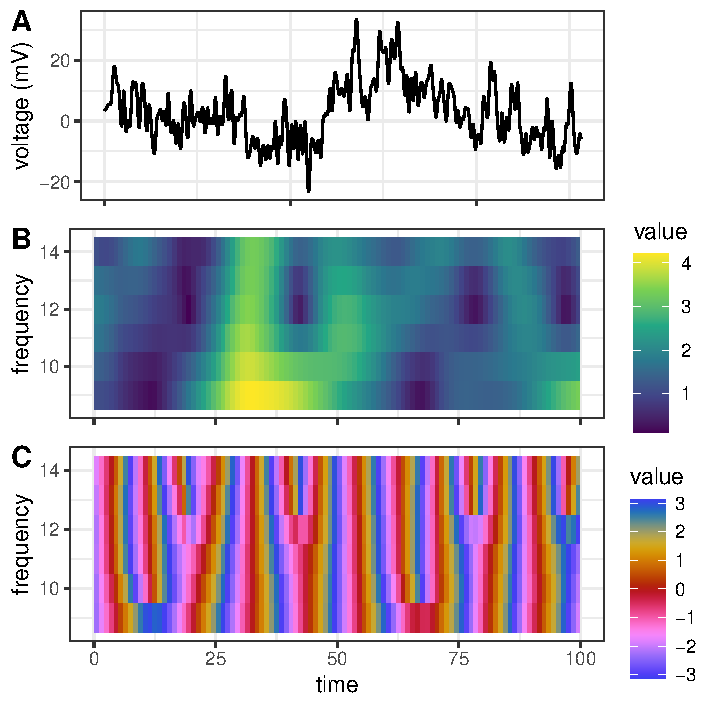
\includegraphics[width=\linewidth]{../stats/results/freqdomain.pdf}
  \caption{Time-frequency plot showing (B) amplitude and (C) phase values. Example frequency domain representation of session 2, participant 1, trial 1, Pz electrode, alpha band (9--14 Hz). The raw data used for the frequency analysis of this trial is shown in (A).}
  \label{fig:freqanalysis}
\end{figure}

\subsection{Time-frequency analysis}
The first step to calculating the phase locking value (PLV), circular
correlation (CCorr) and imaginary part of coherency (ImagCoh) measures consists
of transforming the data into the frequency domain. We do so once every 10
milliseconds for both the alpha band (9--14 Hz) and theta band (4--7 Hz). For
most of the analysis, we use a Hann taper with a frequency dependent window
length of four cycles per window. At least four cycles are recommended by
\textcite{ayrolles_hypyp_2021}. For the lowest frequency of interest (4 Hz),
this results in a window of exactly one second. As a result, the amplitude and
phase of a signal can only be estimated for moments during the trial where half
a second of extra data is available before and after. Because of that, we narrow
the duration of a trial for the purposes of inter-brain synchrony (IBS)
calculation from zero to one second after stimulus presentation exactly.

The result of the frequency analysis is a complex valued Fourier spectrum $x_i$
for each combination of participant, electrode and frequency in the frequency
band. From this spectrum, the amplitudes $r_i$ and phases $\phi_i$ of the input
signal can be extracted by representing the complex values in polar
coordinates. See Figure~\ref{fig:freqanalysis} for a visualization of $r_i$ and
$\phi_i$ of an example signal.

\subsection{Measure definitions}

We compare the signals of homologous electrodes between participants, e.g. we
only compare the signal of the Fz electrode of participant 1 with participant
2's Fz electrode, not with other electrodes. While it is technically possible
to do otherwise, we would lose the ability to conveniently interpret high IBS
as suggestive of similar mental processes in both participants.

The PLV measures whether the difference in the phase of two signals is kept
constant. The PLV measure is defined by \textcite{lachaux_measuring_1999} as
\begin{equation}\label{eq:plv}
\text{PLV} = \cfrac{1}{T}\left|\sum_{t=1}^T e^{i(\phi_i - \phi_j}\right|,
\end{equation}
where $\phi_i$ and $\phi_j$ are the phases of input frequency spectra $x_i$ and
$x_j$ of the different participants. As you can see, the PLV measure is
calculated by averaging along a dimension of size $T$. For this
analysis, we will be averaging over time resulting in one measurement per trial
and frequency. It is also possible to calculate PLV and the other measures
discussed in the current study over trials instead, resulting in a measure of
within-trial IBS. But within the context of \textcite{newman_effects_2021}'s
experiment, how IBS develops over trials is much more interesting. (See
Appendix~\ref{app:task} for more information about
\textcite{newman_effects_2021}'s task.)

While we calculate measures (including PLV) for each whole number frequency
within the frequency band of interest, we are not interested in their
differences within the same band. Instead, we average these values resulting
in a single measure per trial and frequency band. This should contribute to a
more stable estimate. Our PLV implementation was validated against Fieldtrip's
implementation.

\begin{figure}[!htpb]
  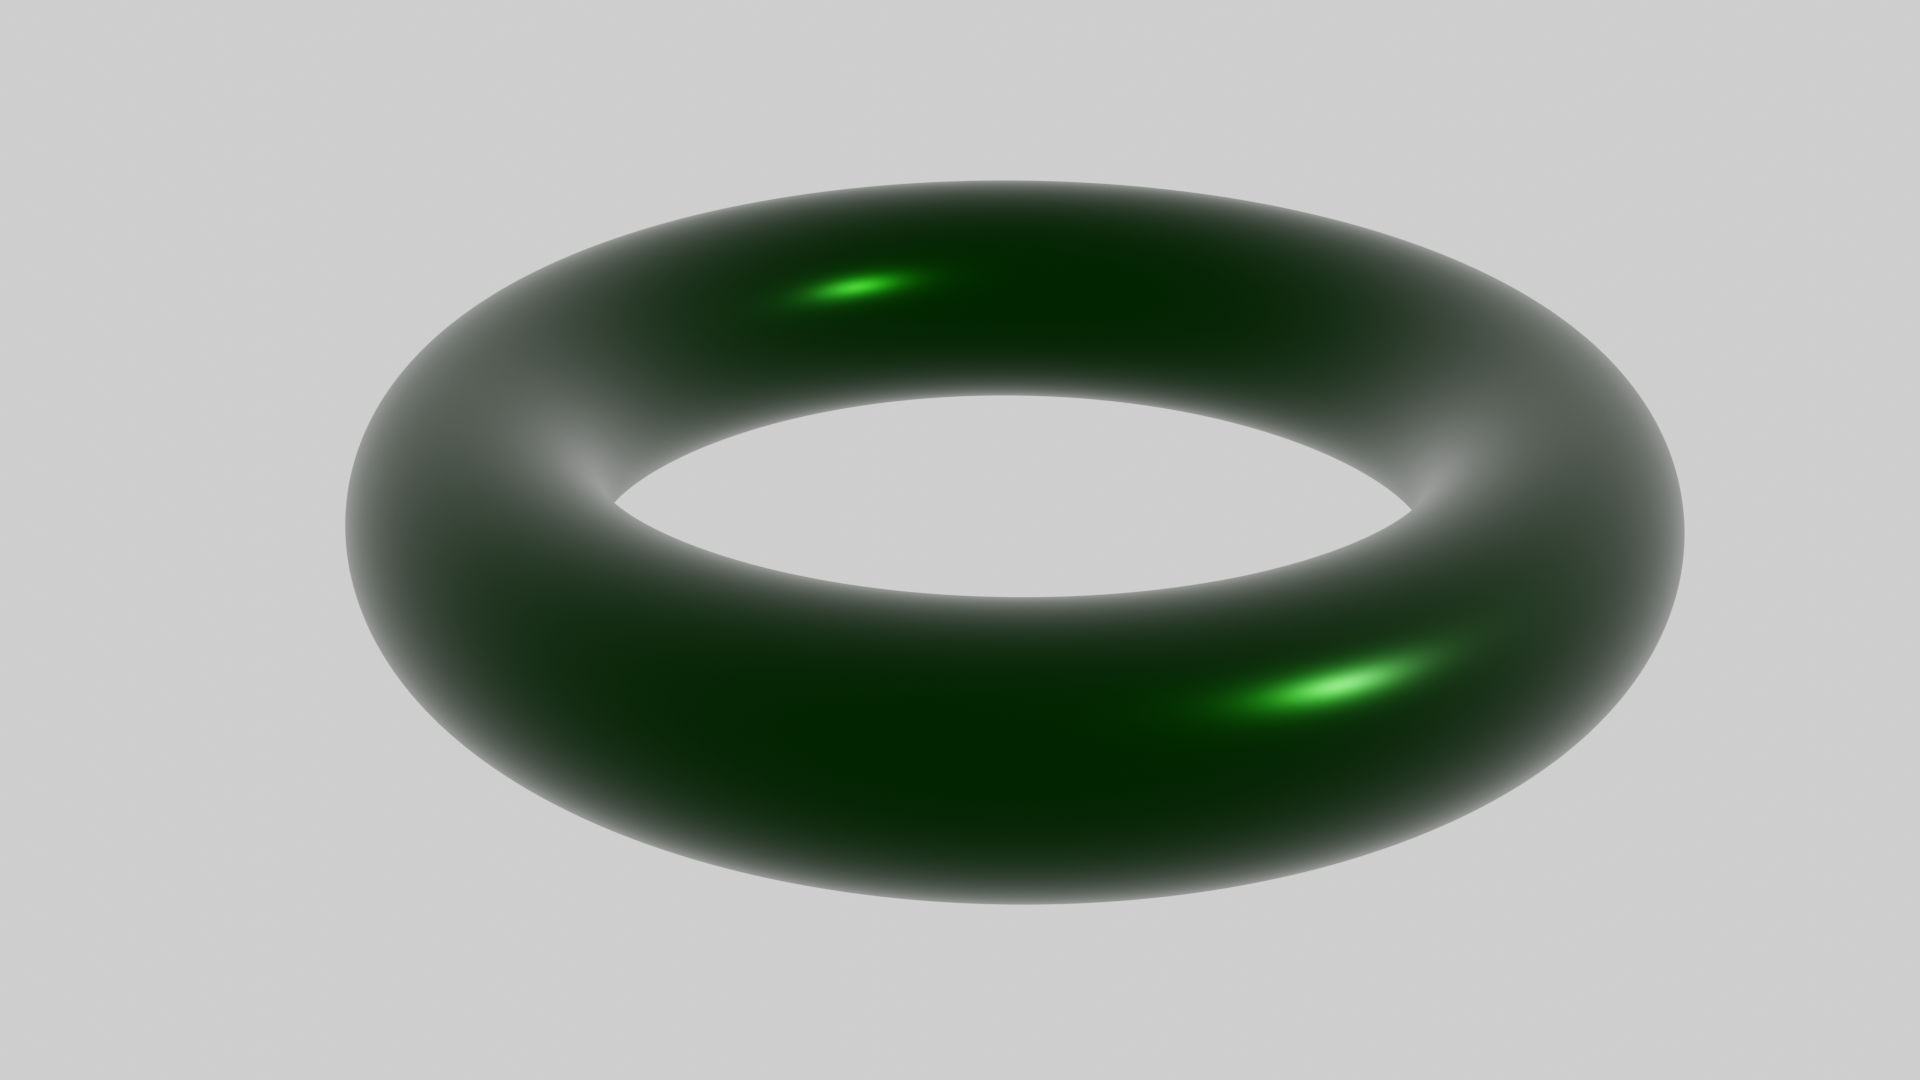
\includegraphics[width=\linewidth]{torus.png}
  \caption{A torus. Bivariate circular data can be thought of as points on a torus. Rendered using Blender \parencite{blender_online_community_blender_2022}.}
  \label{fig:torus}
\end{figure}

CCorr is an analogue of Pearson correlation for angular values
like a phase. It seems to have been first derived by
\textcite{fisher_correlation_1983}, but most recent implementations are based on
the definition by \textcite{jammalamadaka_correlation_1988} which has more
recently been republished in a book \parencite{jammalamadaka_topics_2001}:
\begin{equation}\label{eq:ccorr}
\text{CCorr} = \cfrac{\sum_{t = 1}^T \sin\left(\phi_i - \bar{\phi_i}\right) \sin\left(\phi_j - \bar{\phi_j}\right)}
                {\sqrt{\sum_{t = 1}^T \sin^2\left(\phi_i - \bar{\phi_i}\right) \sin^2\left(\phi_j - \bar{\phi_j}\right)}}.
\end{equation}
Within this equation, $\bar{\phi_i}$ is the circular mean which can be
defined as
\begin{equation}
\bar{\phi_i} = \operatorname{arg} \sum_{t=1}^T e^{\phi_ti},
\end{equation}
where `$\operatorname{arg}$' gives us the angle we get when converting the sum
to polar form. When interpreting normal Pearson correlation coefficients, I
often imagine plotting the two variables of interest against each other. The
coefficient then tells us how close the data points are to lying on a line. With
CCorr values, it is possible to do the same, but instead of a normal
plot you should imagine the data points existing on a torus
\parencite[see also Figure~\ref{fig:torus}]{lee_circular_2010}. Our
implementation of the CCorr measure was inspired by and validated against
the implementation in the CircStat MATLAB toolbox
\parencite{berens_circstat_2009}.

Finally, the ImagCoh measure looks not just at the phase of signals
but also takes into account the amplitude. It is defined by
\textcite{nolte_identifying_2004} as
\begin{equation}\label{eq:imagcoh}
\text{ImagCoh} = \operatorname{Im}\left(\cfrac{S_{ij}}{\sqrt{S_{ii}S_{jj}}}\right),
\end{equation}
where $S_{ij}$ is the crossspectral density of the signals and $S_{ii}$ and
$S_{jj}$ are the autospectral densities of each of the signals. These spectral
densities are estimated directly from the Fourier transformed data $x_i$ and
$x_j$.
\begin{equation}
S_{ij} = \cfrac{1}{T} \sum_{t = 1}^{T} x_i {x_j}^\ast \text{ \parencite{schoffelen_what_2011}},
\end{equation}
where ${x_j}^\ast$ is the complex conjugate of $x_j$. Our implementation of the
ImagCoh measure was validated against Fieldtrip's.

\subsubsection{Statistics}

We use linear mixed effect models with random intercepts over sessions and
electrodes. More complex random effect structures are not supported by the data,
and in some cases including a random intercept for electrodes is not either when
the data is too homogeneous across electrodes. In that case, said random
intercept is left out. Next to any fixed effects of interest, fixed effects of
working memory load, trial and stimulus type were included if they significantly
contributed to the model to account for possibly confounding effects of those.
The models underlying the model comparisons referred to in the text are
reproduced in Appendix~\ref{app:lme}.

\subsection{Software}

All manipulations of the EEG data were performed with Fieldtrip version
20211102 \parencite{oostenveld_fieldtrip_2011} running on MATLAB R2020b. All
IBS measures were implemented from scratch in both MATLAB for use in the
empirical study and R 4.2.0 \parencite{r_core_team_r_2022} for use in the
simulation study. Graphs were generated in R using tidyverse 1.3.2
\parencite{wickham_welcome_2019}, eegUtils 0.7.0
\parencite{craddock_eegutils_2022}, gganimate 1.0.7
\parencite{pedersen_gganimate_2020}, ggh4x 0.2.3
\parencite{van_den_brand_ggh4x_2022}, ggpubr 0.4.0
\parencite{kassambara_ggpubr_2020}, ggvoronoi 0.8.5
\parencite{garrett_ggvoronoi_2022} and pals 1.7 \parencite{wright_pals_2021}.
All statistical tests were performed using R as well, using lme4 1.1.29
\parencite{bates_fitting_2015} for the linear mixed effect models. For the
generalized additive mixed effect models mgcv 1.8.41
\parencite{wood_generalized_2006} was used alongside itsadug 2.4
\parencite{van_rij_itsadug_2020} for plotting those models. To generate
simulated correlated data, faux 1.1.0 \parencite{debruine_faux_2021} was used.
Finally, Python 3.10.8 \parencite{python_software_foundation_python_2021} was
used to train and evaluate classifiers, along with imbalanced-learn 0.1.9
\parencite{lemaitre_imbalanced-learn_2017}, NumPy 1.23.3
\parencite{harris_array_2020}, pandas 1.5.0 \parencite{mckinney_data_2010},
scikit-learn 1.1.2 \parencite{pedregosa_scikit-learn_2011} and SciPy 1.9.1
\parencite{virtanen_scipy_2020}.

Parts of the R and MATLAB code used in this study are available at TODO.

% !TEX root = thesis_draft.tex

\section{Simulation study}

\subsection{Introduction}

While the phase locking value (PLV), circular correlation (CCorr) and
imaginary part of coherency (ImagCoh) measures have been introduced
mathematically, it can be difficult to understand what a certain inter-brain
synchrony (IBS) measure value says about the underlying data. We attempt to
shine some light on the matter using a simulation study.

We introduce a visualization that shows the relation between the phase
components of two EEG signals. For our purposes, one signal from each
participant in the dyad. We then apply this visualization method to simulated
phase data examples. The examples have been chosen such that they result in a
large range of IBS values. This allows us to see what patterns in the
phase data the IBS measures detect, and as a result what relations between the two
signals they are sensitive to (or not).

In these simulations we ignore the amplitude component. This has two reasons: it
is only actually used by the ImagCoh measure, and it would make it harder to
draw any conclusions as it would require more complex visualizations. Finally,
we explain how our approach can be used to perform a power analysis for IBS
experiments.

\subsection{Methods}

\begin{figure}[!htpb]
  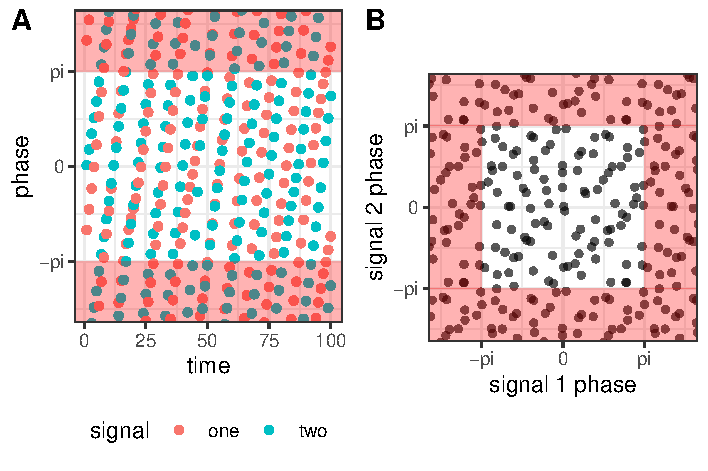
\includegraphics[width=\linewidth]{../stats/results/phases-visualization.pdf}
  \caption{Phase values of both participants in session 2, trial 1 for the Pz electrode at 11Hz. (The trial from Figure~\ref{fig:freqanalysis}.) For this trial, circular correlation = -0.01, phase locking value = 0.033 and imaginary part of coherency = 0.012 (ignoring amplitude values). Shaded areas contain repetitions of the (circular) values. (A): Phase values over time. (B): The same two signals plotted against each other, without time, to show the relation between them. This type of visualization is used throughout this simulation study.}
  \label{fig:phases-visualization}
\end{figure}

As discussed in the general introduction, comparing the relation between two
phase signals requires a space that wraps around in two dimensions. One solution
to this problem is to plot data on a torus (see Figure~\ref{fig:torus}), but
that is not practical for a two-dimensional medium like this report. It would
also result in deformed distances. Instead, we use normal plots, but visualize
the data for 1.5 periods, resulting in a repeated (and differently shaded) area
at the visualization's edges. This makes it easier to imagine the circular
repetition of the data and to spot patterns that would otherwise span the edges
of the plotting area.

We focus on a single session, trial, electrode and frequency at a time. As we
have previusly seen in Figure~\ref{fig:freqanalysis}C, this results in a
one-dimensional phase signal over time for each participant ($\phi$ and $\psi$
respectively). We reproduce these signals in
Figure~\ref{fig:phases-visualization}A, using the y-axis instead of colour to
show their values. If we then get rid of the time dimension, as all discussed
IBS measures do, we can give each phase signal its own axis in
Figure~\ref{fig:phases-visualization}B to make it easier to see the relation
between the two. The resulting plot demonstrates the primary visualization
method used in this study.

The easiest way to simulate this (empirical) phase data is to sample 100 points
from a two-dimensional uniform random distribution with a range of
$[-\pi, \pi)$. We can then calculate the IBS measures on each of these samples.
For the imaginary part of coherency measure, we use a fixed amplitude of one.
When we repeat this process 10~000 times, it results in a distribution of values
for each IBS measure created under the assumption that there is no relation
between the two signals.

While that is useful, completely random signals are unlikely to elicit the full
range of IBS values. To be able to generate signals for any measure
value, we created Algorithm~\ref{alg:optimize-measures}.

\begin{algorithm}
  \caption{Generates random phase data examples that minimize an evaluation function $f$ using a combination of global and local search.}
  \begin{algorithmic}
  \Require $f(\phi, \psi) \to \mathbb{R}$ \Comment{the evaluation function to minimize}
  \State repetitions $\gets$ the amount of global search iterations
  \State start $\gets$ the initial amount of data points in the sample (should be $\geq$ end)
  \State end $\gets$ the amount of data points in the sample after local search finishes
  \\
  \State best $\gets \infty$
  \State result $\gets [~]$
  \For{'repetitions' amount of iterations} \Comment{the global search part}
    \State $\phi, \psi \gets$ a 2D uniform random sample of length `start' and range $[-\pi, \pi)$
    \While{cur > end} \Comment{the local search part}
      \For{$i \in 1 \ldots \text{length of } \phi$}
        \State $\phi'_i, \psi_i \gets \phi, \psi$ without the $i$th values
        \State $e_i \gets f(\phi'_i, \psi'_i)$
      \EndFor
      \State $i \gets \text{argmin}(e_i)$
      \State $\phi, \psi \gets \phi'_i, \psi'_i$
    \EndWhile
    \If{$f(\phi, \psi) < \text{best}$}
      \State best $\gets f(\phi, \psi)$
      \State result $\gets [\phi~\psi]$
    \EndIf
  \EndFor
  \State\Return result
  \end{algorithmic}
  \label{alg:optimize-measures}
\end{algorithm}

Algorithm~\ref{alg:optimize-measures} finds example signals that minimize an
evaluation function $f(\phi, \psi)$. It uses a combination of global and local
search. The global search part of the process generates multiple random signals
and picks the ones that minimizes the evaluation function. The local search part
of the process optimizes each candidate before evaluation by removing a number
of `outliers' (as determined by the evaluation function), one at a time. By
varying the input parameters, it is possible to trade-off between the (unbiased,
but unlikely to cover the whole range) global search process and the (biased,
but more flexible) local search process.

We apply Algorithm~\ref{alg:optimize-measures} in two tasks.

First, we use it to generate examples that have CCorr and ImagCoh values close
to $-1, -0.75, \ldots, 0.75$ and $1$. And the same for the PLV values
$0, 0.125, \ldots, 0.875$ and $1$. To approximate values, we use an L2 loss
function as the evaluation function. E.g. to get a CCorr value of
$-0.75$ the evaluation function is
\begin{align}
  f(\phi, \psi) = \left(CCorr(\phi, \psi) - (-0.75)\right)^2,
\end{align}
where $CCorr$ is as defined in Equation~\ref{eq:ccorr}.

Secondly, to further contrain the examples and to see where the IBS measures
differ, we use evaluation functions that constrain the measures in different
ways simultaneously. For example, when minimizing the evaluation function
\begin{align}
  f(\phi, \psi) = 1 - CCorr(\phi, \psi) + |ImagCoh(\phi, \psi)| + PLV(\phi, \psi),
\end{align}
we obtain example signals with a positive CCorr value, a (close to) zero
ImagCoh value and a low PLV value. We generate example signals for all possible
constraint permutations. The $PLV$ and $ImaghCoh$ definitions are given in
Equations~\ref{eq:plv}~and~\ref{eq:imagcoh}.

\subsection{Results}

\begin{figure}[!htpb]
  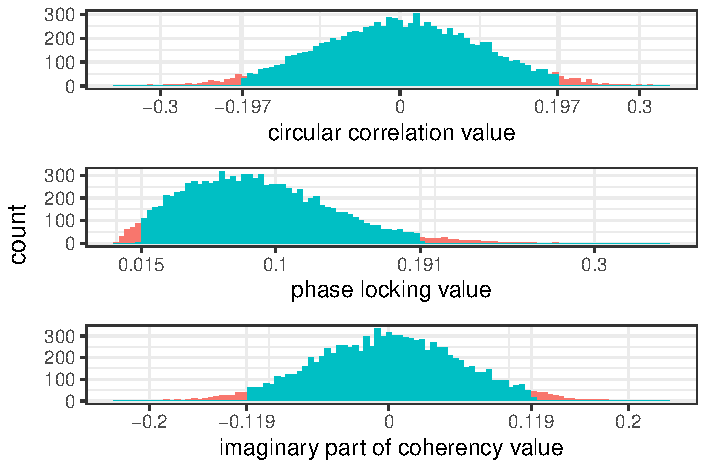
\includegraphics[width=\linewidth]{../stats/results/simulation_null.pdf}
  \caption{A histogram of inter-brain synchrony values calculated on 10~000 pairs of uniform random signals. It shows inter-brain synchrony values typical for when the underlying signals are unrelated. The central 95\% of the data is shown in blue.}
  \label{fig:simulation_null}
\end{figure}

In Figure~\ref{fig:simulation_null}, we see the distribution of IBS values
when the underlying signals are completely random. We see that the distributions
for the CCorr and ImagCoh values are symmetric and centered around their middle
value of zero. We observe a skewed distribution for the PLV measure values, most
likely because the values are all close to the minimum value the measure can
take (i.e. zero). It will be virtually impossible to distinguish an effect
that has an IBS value in the high density part of the shown distributions
from noise.

In Figure~\ref{fig:simulation_force_individually}, we see the phase components
of example signals for the whole range of CCorr, ImagCoh and PLV measure values.
Finding ImagCoh examples was harder than finding examples for the other
measures, resulting in different input parameters for
Algorithm~\ref{alg:optimize-measures} being required to cover the whole range.
These parameters can be found in Table~\ref{tab:force_individually_params}.

\begin{landscape}
  \begin{figure}
    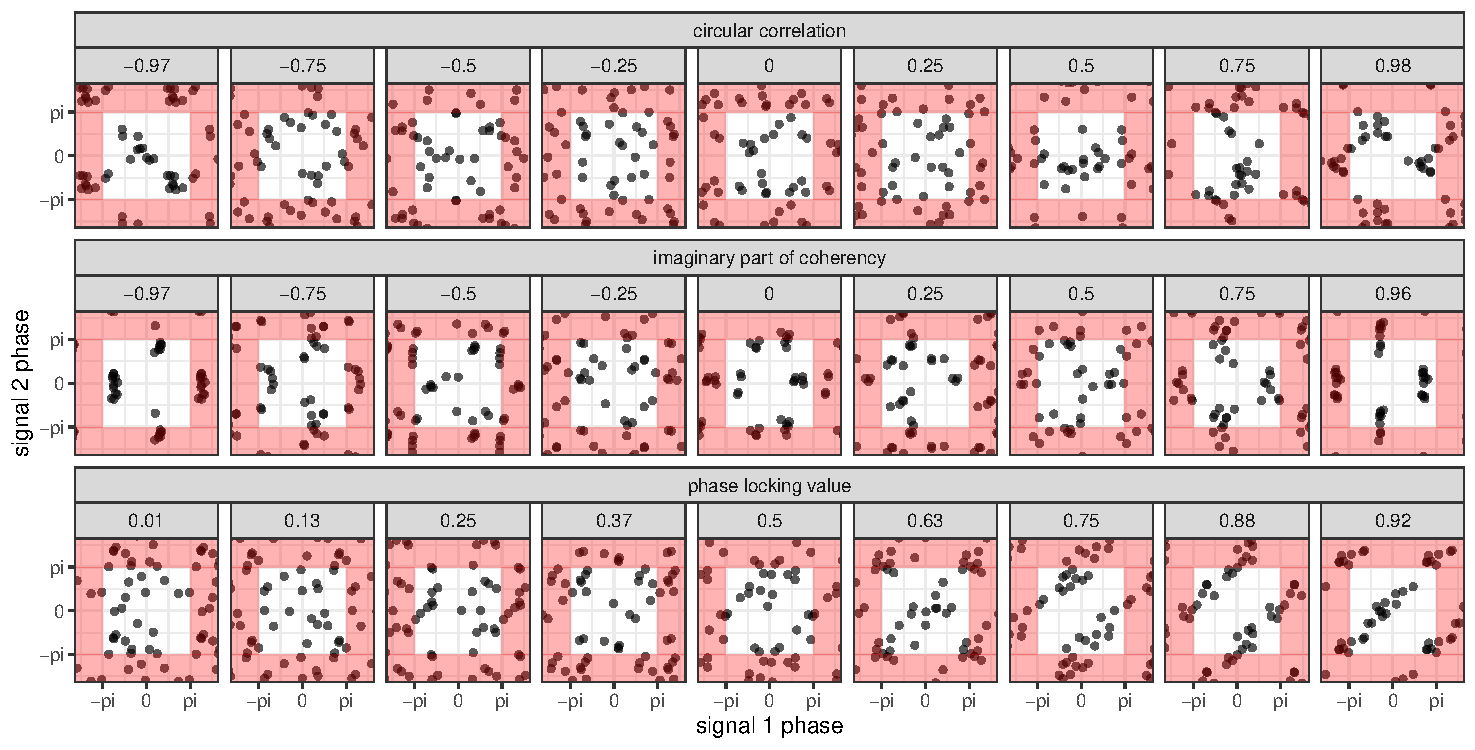
\includegraphics[width=\linewidth]{../stats/results/simulation_force_individually.pdf}
    \caption{Simulated examples for the whole range of inter-brain synchrony measure values. As in Figure~\ref{fig:phases-visualization}, shaded areas contain repetitions of the (circular) values. A high phase locking value requires a positive linear relation between signals. For a high circular correlation or imaginary part of coherency, multiple clumps suffice. But interestingly, while the simulation finds random noise examples for PLV and CCorr values of zero, the ImagCoh is assigned a clumped example instead.}
    \label{fig:simulation_force_individually}
  \end{figure}
\end{landscape}

\begin{table}[!htbp]
  \caption{Parameter values of Algorithm~\ref{alg:optimize-measures} used to generate Figure~\ref{fig:simulation_force_individually}.}
  \label{tab:force_individually_params}
  \begin{tabular}{l r r}
    \hline
    Parameter   & circular correlation \& phase locking value & imaginary part of coherency\\\hline
    repetitions &      1000 &          20\\
    start       &        40 &         200\\
    end         & (/2 =) 20 &  (/10 =) 20\\\hline
  \end{tabular}
\end{table}

The examples show a few clear trends. First of all, an increase in PLV seems to
lead to a more positive and linear relation between the phase components of the
example signals. For the other measures, higher (and lower) IBS values seem
to lead to the formation of clumps, i.e. patterns where a lot of the phase
components are approximately constant. Surprisingly, while the other measures
seem to converge on a (at first glance) random noise example for IBS values
of zero, which is in line with our findings in Figure~\ref{fig:simulation_null},
this is not the case for the ImagCoh measure. There, the
central example is clumped just like the examples at the tails.

To see whether these examples are typical or just the first configuration
Algorithm~\ref{alg:optimize-measures} finds, we further constrain the examples
by forcing them into configurations that contrast the IBS measure values.
Figure~\ref{fig:simulation_local_search} shows these examples. As this
optimization problem is harder, an optimal solution is not always found. Because
of that, the size of the error is shown as well, which is at the same scale as
the IBS values themselves. While the total error occasionally surpasses
0.5, the error is in practise divided up among measures. So while the examples
might not match the target IBS values exactly, they are never so far off as
to become misleading.

To generate Figure~\ref{fig:simulation_local_search}, 100 global search
repetitions were used. The local search started with 100 samples, and reduced
that to 20 samples.

\begin{landscape}
  \begin{figure}
    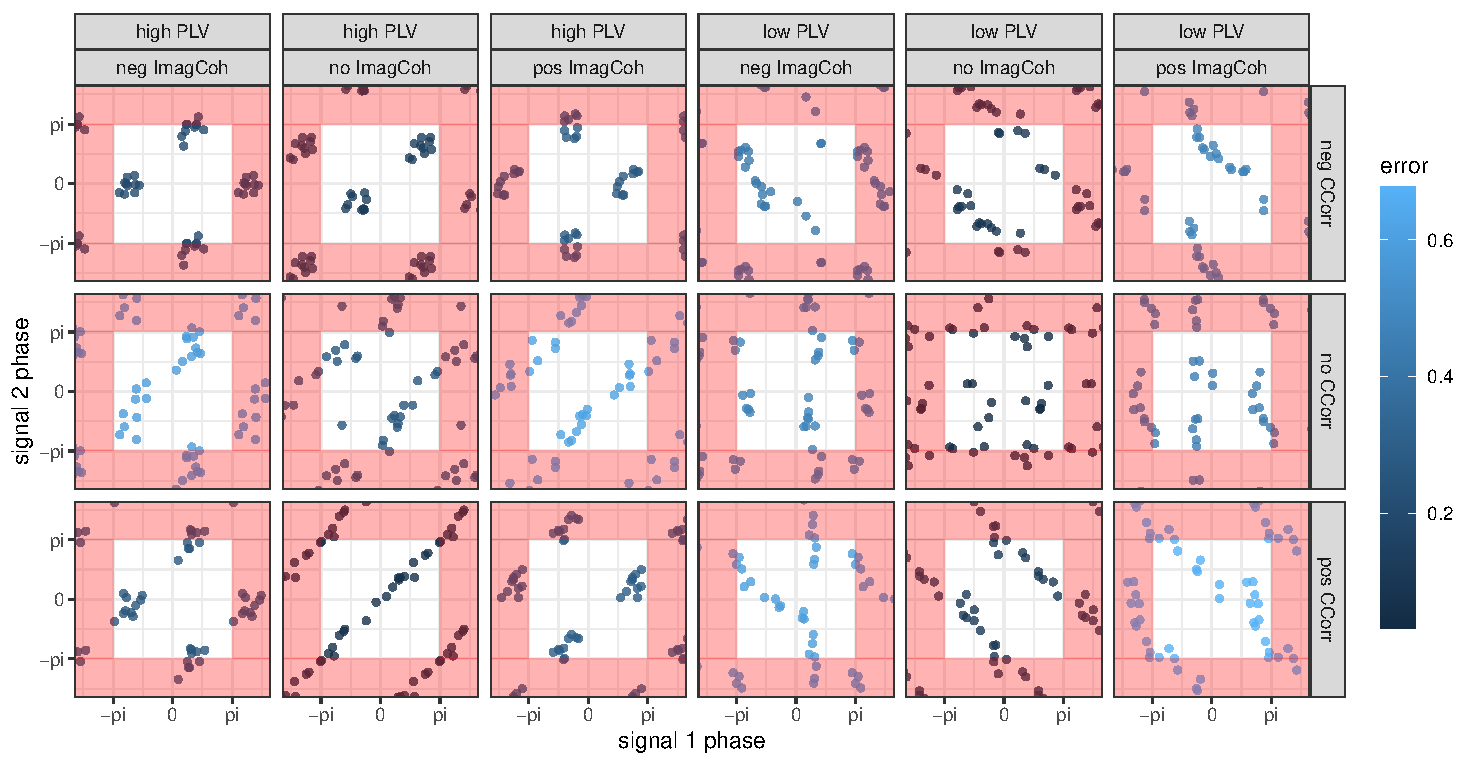
\includegraphics[width=\linewidth]{../stats/results/simulation_local_search.pdf}
    \caption{Simulated examples that minimize (low phase locking value, negative imaginary part of coherency, negative circular correlation), maximize (high PLV, positive ImagCoh, positive CCorr) or zero out (no CCorr, no ImagCoh) IBS values simultaneuously. Light blue dots indicate the example is not perfect (fulfilling the ImagCoh requirement is often most difficult), while black dots indicate all constraints were met perfectly.}
    \label{fig:simulation_local_search}
  \end{figure}
\end{landscape}

We see that PLV is not sensitive to negative linear trends (as opposed to
positive ones) at all. This is exploited in the right side of
Figure~\ref{fig:simulation_local_search}, as depending on the exact
configuration the CCorr and ImagCoh measures
are sensitive to negative trends. We further see confirmation that the imaginary
part of coherency can reach a value of zero just fine with an (apparently)
random example (the `low PLV, no ImagCoh, no CCorr' condition). Also, it is
interesting to point out that the ImagCoh is sensitive to
the phase components of signals being constant in one dimension but not in the
other, contrary to the CCorr. (See e.g. the `low PLV, no CCorr'
conditions with negative or positive ImagCoh values).
Next, it is worth noting that a configuration with a seemingly negative trend
(`low PLV, no ImagCoh, pos CCorr') results in a positive CCorr
value. Finally, to the eye immediately apparent trends are not always picked up
on by the ImagCoh measure. (E.g. the two `pos CCorr, no ImagCoh' conditions.)

\subsection{Discussion}

The lack of response of the PLV measure to a clear negative relation between the
phase components of the input signals is not unexpected, as it only reports
whether the phases are directly coupled, not if one of them can be used to
predict the other \parencite{burgess_interpretation_2013}. But it is a downside,
as you would most likely want to detect such effects in IBS experiments.

Similarly, we saw that the ImagCoh measure failed to
sometimes detect trends. That might be because it is designed not to detect
signals that are perfectly in phase, as a way to (originally) prevent spurious
effects due to volume conduction \parencite{nolte_identifying_2004}. But these
simulations suggest that the cost of that might be too high. On the other hand,
it is important to keep in mind that these simulations are not a level playing
field for the ImagCoh measure: amplitude components of the
signal on which it is normally dependent are held constant.

In the end, the CCorr values seem the least surprising
given the studied examples, although the direction of any relations (i.e.
whether the correlation coefficient is positive or negative) should probably not
be relied on.

\subsubsection{Power analysis for inter-brain synchrony experiments}

Taking a step back, it is worth pointing out that
Algorithm~\ref{alg:optimize-measures} is a very flexible method to generate
phase component data for a target IBS value. It could potentially be used to
perform an up-front power analysis for a test in an IBS experiment. The steps
would be as follows:

\begin{enumerate}
  \item Choose a target effect size. That is, what IBS value would you
  expect your experiment to find? The simulations in this section give you some
  guidance on what would be reasonable values, but ideally the target value
  would be decided based on what other similar studies found.
  \item For a range of sample sizes, repeatedly simulate the outcome of your
  test using the Monte Carlo method
  \parencite[p.~150 gives a nice introduction]{cohen_empirical_1995} as
  follows:
  \begin{enumerate}
    \item Use Algorithm~\ref{alg:optimize-measures} to generate fake trials
    for your IBS value of choice. By varying the trade-off between global- and
    local search part of the algorithm, you have some control over the variation
    around your target IBS value. Ideally, you would again use this to match
    the variation found in other similar studies.
    \item Perform your test on the simulated data, recording the outcome.
  \end{enumerate}
  \item Use the collected outcomes to estimate the power of your test for each
  sample size.
\end{enumerate}

A downside of this method, and in fact of this simulation study in general, is
that the local search part of Algorithm~\ref{alg:optimize-measures} introduces
a bias due to the way it removes outliers. After all, removing them one at a
time is just one of many possible approaches. While the results seem reasonable
looking at the graphs, it could be that some examples we observe are in fact
not typical but artifacts of the process used to generate them. This could
for example perhaps explain the clumps in the ImagCoh plot
in the very middle of Figure~\ref{fig:simulation_force_individually}.

% !TEX root = thesis_draft.tex

\section{Varying time-frequency analysis methods}

\subsection{Introduction}

Inter-brain synchrony (IBS) values are calculated on a frequency domain
representation of the original signals. Obtaining this frequency domain
representation requires making some methodological choices: you need to choose
a window of interest, a calculation method and a resolution. We assess how these
choices affect the final IBS values.

Ideally, the IBS values should be robust to slight changes in these parameters.
For the window of interest case, IBS values could presumably vary a bit as
the window could include or exclude cognitive processes that take a while to
start after the stimulus. But the other parameters are just technical details of
the time-frequency analysis process and should not have a big effect on the IBS
values when reasonably chosen.

\subsection{Methods}

To assess the effect of different windows of interest on the
results, we repeat the main frequency analysis using a window of half a second
before to one second after stimulus presentation, making full use of each
available pre-processed data point. To determine the effect of different
frequency analysis methods on the final results, we also repeat the (alpha band)
analysis using multitapers instead of a Hann taper. To find whether there is an
effect of resolution, we perform the frequency analysis both more often (for
each original data point, i.e. 512 times per second or approximately every 2 ms)
and less often (once every 20 ms). None of these variations are extreme, and all
could have been reasonably chosen for the main experiment instead.

For each of these variations, we first compare the averaged IBS values by
plotting the data and assess the significance using a linear mixed effect model.
If those do not show a difference at first glance, we further assess possible
differences in the underlying data structure by calculating correlations between
the values for different conditions and (where necessary) by plotting the data.
Correlations are calculated for each session, Fisher transformed
\parencite{fisher_frequency_1915}, averaged and transformed back.

\subsection{Results}

\subsubsection{Frequency analysis window size}

\begin{figure}[!htpb]
  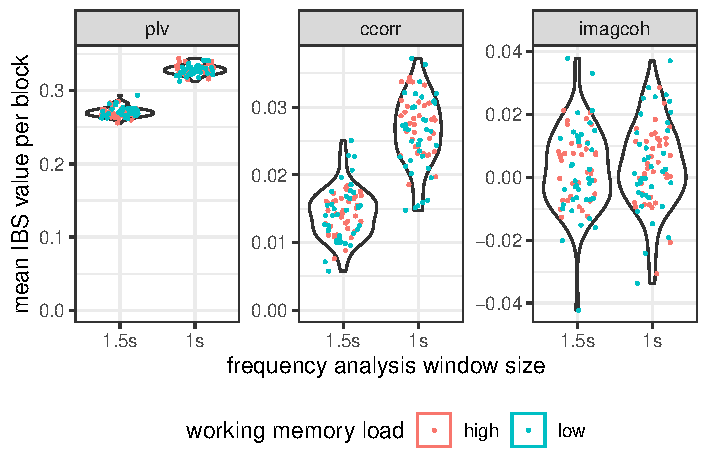
\includegraphics[width=\linewidth]{../stats/results/winsize.pdf}
  \caption{(Mean) alpha band inter-brain synchrony values are sensitive to different time windows of interest within a trial. The 1s window starts at the presentation of the stimuli, while the 1.5s window starts half a second earlier during fixation. Working memory load has no effect. Finally, the (mean) circular correlation and imaginary part of coherency values are both very close to zero considering they are on a scale from -1 to 1. The phase locking value is on a 0-1 scale.}
  \label{fig:winsize}
\end{figure}

We tested the effect of window size on IBS values by calculating the IBS
measures on overlapping windows of 1s and 1.5s respectively. Contrary to our
initial expectations, we found IBS values to be sensitive to changes
in frequency analysis window size. See Figure~\ref{fig:winsize}. The phase
locking value (PLV) significantly decreased when the larger window was used
($\chi^2$(1) = 29984, p < 0.001, $\Delta$AIC = 29982, $\Delta$BIC = 29971) and
so did the circular correlation (CCorr; $\chi^2$(1) = 1071, p < 0.001, $\Delta$AIC = 1069,
$\Delta$BIC = 1058), but no significant effect was found for the imaginary part
of coherency values (ImagCoh; $\chi^2$(1) = 2.27, n.s., $\Delta$AIC = 0.27,
$\Delta$BIC = 10.66).

\subsubsection{Frequency analysis taper}

\begin{figure}[!htpb]
  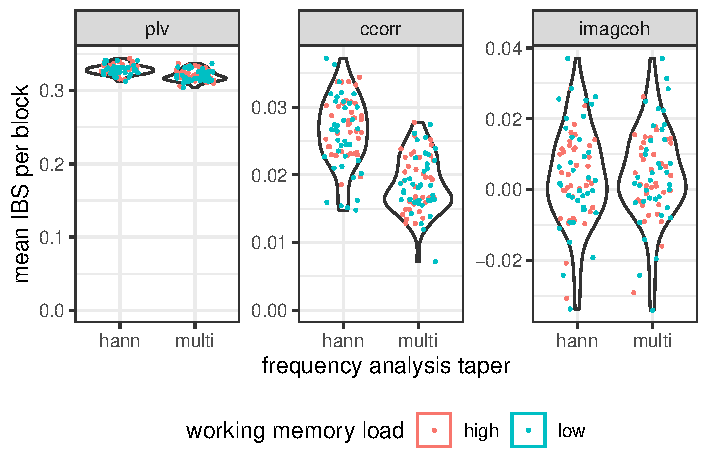
\includegraphics[width=\linewidth]{../stats/results/freqmethod.pdf}s
  \caption{Choice of taper matters when calculating (mean) `phase locking value', `circular correlation' and `imaginary part of coherency' inter-brain synchrony values for the alpha band. Working memory load has no influence.}
  \label{fig:freqmethod}
\end{figure}

\begin{figure}[!htpb]
  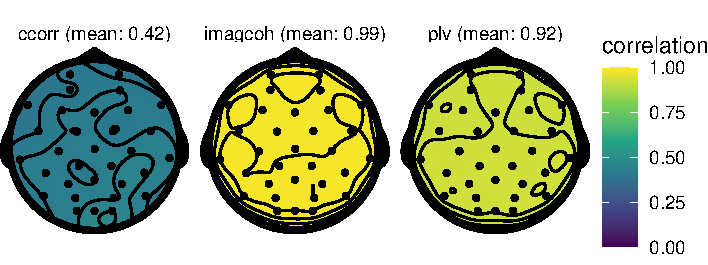
\includegraphics[width=\linewidth]{../stats/results/freqmethodcorr.pdf}
  \caption{When calculating phase locking value and circular correlation measures, the choice of taper alone can lead to inter-brain synchrony values different enough that they do not perfectly correlate with each other. Imaginary part of coherency values are less affected than circular correlations and phase locking values.}
  \label{fig:freqmethodcorr}
\end{figure}

To see the effect of taper choice on the frequency analysis, we compared the
IBS values obtained from spectra generated using a Hann taper and a multitaper.
As you can see in Figure~\ref{fig:freqmethod}, there is an effect of taper
choice on PLV synchrony values ($\chi^2$(1) = 626, p < 0.001, $\Delta$AIC = 624,
$\Delta$BIC = 614) and CCorr synchony values. ($\chi^2$(1) = 452, p < 0.001,
$\Delta$AIC = 450, $\Delta$BIC = 440). In both cases, the IBS value decreases a
bit when multitapers are used. Again, there is no significant effect on
ImagCoh synchrony values ($\chi^2$(1) = 0.51, n.s., $\Delta$AIC = 1.49,
$\Delta$BIC = 12.4). When we compare how values calculated using the different
methods correlate (Figure \ref{fig:freqmethodcorr}), we again see that IBS value
calculation is sensitive to choice of taper contrary to our hypothesis. The
CCorr measure is especially affected with a mean correlation of 0.42 across
sessions and electrodes.

\subsubsection{Frequency analysis resolution}

\begin{figure}[!htpb]
  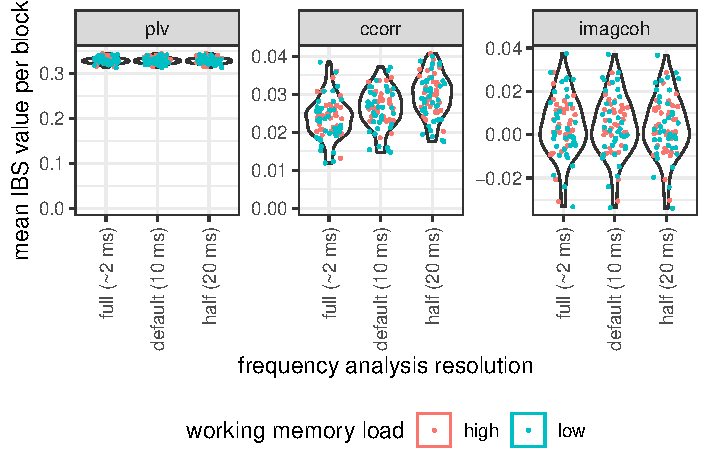
\includegraphics[width=\linewidth]{../stats/results/resolution.pdf}
  \caption{Mean inter-brain synchrony values do not appear to vary much with resolution, with the exception of a slight effect on circular correlation values.}
  \label{fig:resolution}
\end{figure}

\begin{figure}[!htpb]
  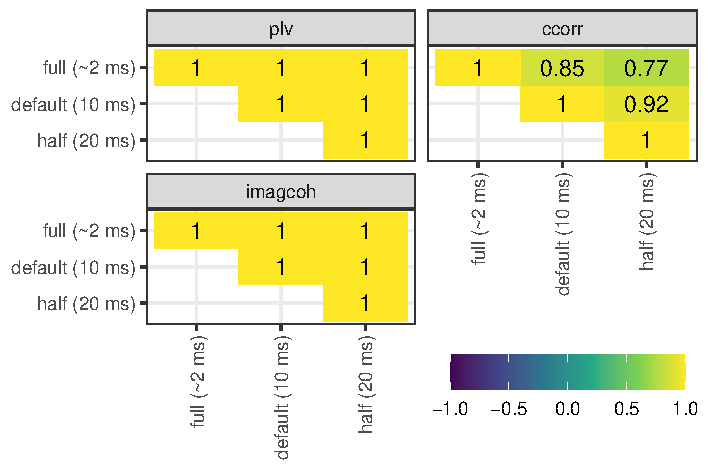
\includegraphics[width=\linewidth]{../stats/results/resolutioncorr.pdf}
  \caption{The phase locking value and imaginary part of coherency measures are robust to being calculated on frequency spectra of different resolutions. Circular correlation values, in contrast, will not correlate perfectly when comparing values across resolutions. Figure~\ref{fig:resolutionapp} shows the full underlying data for the CCorr case where $r$ = 0.77.}
  \label{fig:resolutioncorr}
\end{figure}

We now turn to a less discussed parameter of the frequency analysis: the
resolution of the resulting spectrum. At first sight, there does not appear to
be an effect of resolution on IBS values (Figure~\ref{fig:resolution}). When
using the resolution as a continuous parameter ($\frac{1000}{512}$ ms, 10 ms or
20 ms), statistics confirm this for the PLV ($\chi^2$(1) = 0.145, n.s.,
$\Delta$AIC = 1.85, $\Delta$BIC = 13.2) and ImagCoh ($\chi^2$(1) = 0, n.s.,
$\Delta$AIC = 2.0, $\Delta$BIC = 13.3) measures, but report a significant
positive (though small) effect of resolution on CCorr synchrony values
($\chi^2$(1) = 7.4, p < 0.01, $\Delta$AIC = 5.4, $\Delta$BIC = -5.9).

Looking into it further, we see that CCorr values in fact
correlate much worse across resolutions than the other measures
(see Figure~\ref{fig:resolutioncorr}). This is unexpected when varying such a
`boring' parameter as resolution, which you normally do not think twice about
when choosing it.


\subsection{Discussion}

An effect of window size was found for the CCorr and PLV measures, but not for
the ImagCoh measure. In hindsight, the effect of window size is not that
surprising, as all measure definitions weigh each data point equally and one
third of the data is new for the 1.5s window of interest. Still, as all IBS
present in the short window is also present in the longer window, we would not
expect any effects to change direction, especially as the extra half second is
time in which the participants are `only' watching the fixation point. This
indeed seems to be the case.

The lack of an effect on the ImagCoh measure could mean that the underlying
functional (dis)similarities that the other measures now pick up on are in phase
in both signals. But it could also just indicate a lack of sensitivity of the
ImagCoh measure.

Using multitapers also changed CCorr and PLV values. This could
be because multitapers are ill suited to performing a frequency analysis of
low-frequency data \parencite[p.~203]{cohen_analyzing_2014}. (Which the alpha
band (9--14 Hz) data used for this experiment is.) But that does not explain why
the CCorr and PLV measures are again more affected than the ImagCoh measure.
Especially the CCorr value with a mean correlation when comparing tapers of only
0.42 across sessions and electrodes (Figure~\ref{fig:freqmethodcorr}).

As expected, no effect of resolution was found for the PLV and ImagCoh measures.
In contrast, the CCorr values are not stable when calculated for different
resolutions. While you could still argue that the variance was reasonable for
the multitaper case, it seems conceptually bad for a change in sampling rate to
have a big effect on an IBS value when the underlying data has not
changed. So it is worth discussing the big variance introduced by the CCorr
measure in more detail.

\subsubsection{Stability of circular correlation synchrony values}

We found the CCorr values to change quite a bit when only small
changes to the frequency analysis process where made. Apparently, contrary to
PLV and ImagCoh, the values do not converge to a single stable value. This is
surpising, because \textcite{burgess_interpretation_2013} previously found CCorr
to be more robust than other measures. \textcite{pauen_circular_2013} also found
it to at least not perform worse than PLV.

\begin{algorithm}[!htpb]
  \caption{Calculates a robust circular correlation coefficient. Based on \textcite{mahmood_robust_2022}'s work, using the (univariate) dispersion measure from \textcite[p.~28]{pewsey_circular_2013}.}
  \begin{algorithmic}
  \Require $\phi, \psi$ \Comment The input signals (phases).
  \State $n \gets \text{length of }\phi$
  \State $n' \gets n \cdot 0.95$ \Comment How many data points to keep?
  \While{$n > n'$}
    \For{$i \in 1 \ldots n$}
      \State $d_i \gets \sum\limits_{j = 0}^n \text{dist}(\phi_i, \phi_j) + \text{dist}(\psi_i, \psi_j)$
    \EndFor
    \State $i \gets \text{argmax}(d)$ \Comment The point that maximizes the distances.
    \State remove $\phi_i$ and $\psi_i$ from $\phi$ and $\psi$ respectively
    \State $n \gets n - 1$
   \EndWhile
   \State\Return $\text{CCorr}(\phi, \psi)$ \Comment As defined in Equation~\ref{eq:ccorr}.
  \end{algorithmic}
  \label{alg:robust}
\end{algorithm}

When investigating why the CCorr varies this much, we
hypothesised it could be overly influenced by outliers.
\textcite{mahmood_robust_2022} proposes a robust version of the CCorr measure
which removes values that ``lie far away from the majority of the circular data
based on the circular geometry theory''.
\citeauthor{mahmood_robust_2022} shows using simulations that his `trimmed
robust circular correlation' measure succesfully reduces the influence of
outliers. That makes it ideal to test our hypothesis. But sadly, not enough
information is provided to unambiguously reproduce
\citeauthor{mahmood_robust_2022}'s method. While `lying far away' is
well-defined for univariate circular data using the dispersion measure
\parencite[p.~26]{pewsey_circular_2013}, robust correlations need to have a way
of detecting bivariate outliers \parencite[p.~12]{maronna_robust_2019} as points
can be outliers while not being extreme in any dimension by itself. To the best
of my knowledge, such methods have only been published for normal correlations
\parencite[chapter~6]{bebbington_method_1978,shevlyakov_robust_2010,maronna_robust_2019}, not circular ones.
As a result, it is likely that \citeauthor{mahmood_robust_2022} instead only
considered outliers that are isolated in a single dimension. Working with this
assumption, we defined the robust circular correlation as given in
Algorithm~\ref{alg:robust}.

The resulting algorithm is slow, so it was only applied to the data sets
obtained using the standard frequency analysis resolution (10 ms) and half the
resolution (20 ms). It results in circular correlation values higher (around
0.11) than those found previously (around 0.03; Figure~\ref{fig:resolution}).
When correlating the IBS values for the different resolutions, we get a (mean)
correlation of 0.87, which is close to the value of 0.92 we got for normal
CCorr (Figure~\ref{fig:resolutioncorr}). But as it is still not
`1', our robust circular correlation measure clearly did nothing to resolve the
circular correlation stability issue. Apparently, outliers are not the problem.

\begin{figure}[!htpb]
  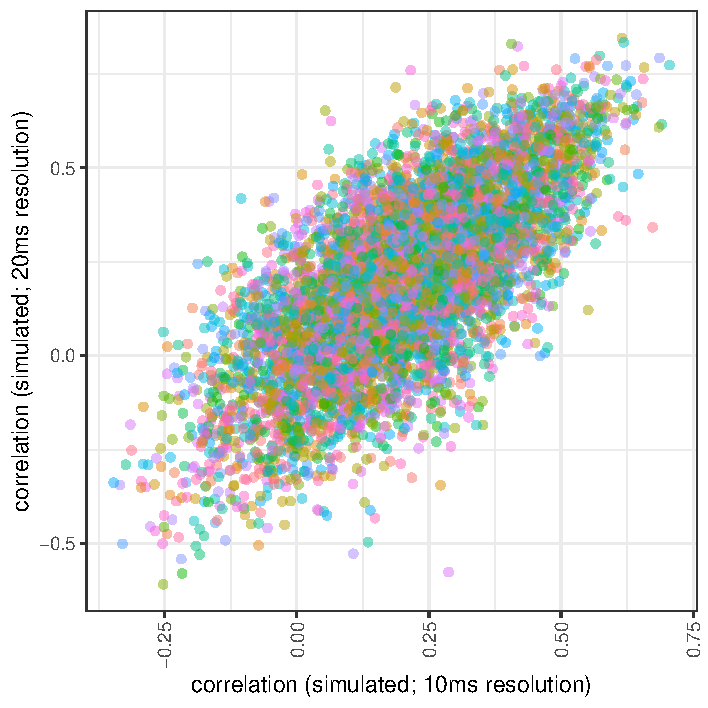
\includegraphics[width=\linewidth]{../stats/results/corsimulation.pdf}
  \caption{The correlation of simulated (correlated) normal data before and after downsampling. Simulates a single session with 32 electrodes (each represented by a different color) for 180 trials. The result matches the emperical data in Figure~\ref{fig:resolutionapp} quite well. This illustrates that the circular correlation stability issue also exists for normal correlations.}
  \label{fig:corsimulation}
\end{figure}

As sampling at half the resolution is equivalent to just leaving out every
second data point, the issue is also unlikely to be caused by more sophisticated
frequency analysis issues like spectral leakage. Instead, after further
investigation, the problem seems to be inherent to correlation measures. This is
most easily demonstrated with a simulation. We replace the CCorr measure with a
Pearson correlation, and the underlying phase signals by data drawn from a
multi-variate normal distribution while making sure the signals are somewhat
correlated. We also calculate correlations after downsampling our `signals' by
half. The result can be seen in Figure~\ref{fig:corsimulation}. Clearly, the
correlation ($r=0.72$) between CCorrs of different resolutions is not perfect
when using normal correlations to simulate them either.

On the one hand, this is good news. Normal correlations are not fundamentally
flawed, so there is no reason not to use the CCorr measure either. On the other
hand, it cannot be denied that CCorr values are less stable than PLV or ImagCoh
values. As such, more care is required when interpreting raw values, as we will
do in the time course analysis section. Permutation tests are an elegant
solution to the problem: as they encounter the variation issue also during null
distribution construction, it is automatically taken into account when
determining the final p-value.

% !TEX root = thesis_draft.tex

\section{Permutation test analysis}
\label{sec:permutationtest}

\subsection{Introduction}

At this point it is clear how we calculate the raw inter-brain synchrony (IBS)
values, and we have some ideas on how to interprete them. But to
explore how they integrate in a full analysis, we need some task-related
analysis goals to cut our teeth on.

\subsubsection{Task-related research questions}
We decided to determine whether there is an effect of cooperation in
\textcite{newman_effects_2021}'s coordination task on IBS. Assuming there is an
effect, we want to know:

\begin{APAenumerate}
  \item Is the effect of cooperation merely task-dependent (e.g. due to stimuli
  or motor responses), or due to actual interaction within the dyad?
  \item Is there also an effect of the study's manipulation (i.e. varying
  working memory load) on IBS, and how does it develop over time?
  \item Is it possible to predict for new EEG data whether cooperation was
  succesful using just the IBS values?
\end{APAenumerate}

Based on the hyperscanning studies discussed in the introduction, we hypothesize
regarding our task-related research questions that more cooperation will lead to
higher synchrony. We also expect such an effect to not just be caused by the
task but also by the interaction itself. And as a consequence, we expect
prediction of accuracy (i.e. succesful cooperation) on the basis of newly
collected EEG data to also be possible. We expect IBS to vary over time, as at
some point we expect participants to stumble upon a cooperation strategy.
Finally, we hypothesize high working memory load to be detrimental to IBS
because of \textcite{maehara_i_2011,newman_effects_2021}'s behavioural results.

While most of the task-related questions we plan to answer have an exploratory
nature, we also have one directly testable hypothesis: we expect IBS in frontal
and temperoparietal areas in the alpha band \parencite{newman_effects_2021}.
This hypothesis is based on the findings of
\textcite{van_vugt_inter-brain_2020}. They found ``frontal alpha oscillations''
during ``moments of agreement'' in monastic debate. And also on the findings of
\textcite{hu_inter-brain_2018}, who found higher (phase locking value) synchrony
in the alpha band in centro-parietal regions during high cooperation than low
cooperation.

\subsection{Methods}

The task-dependent and dyad-dependent effects on IBS are tested separately,
the former by running a permutation test against shuffled samples and the latter
by running a permutation test against virtual dyads assembled from random
participants that never performed the task together.

% NOTE: these are included early because a lot of figures follow in a small
% amount of text
\begin{figure}[!htpb]
  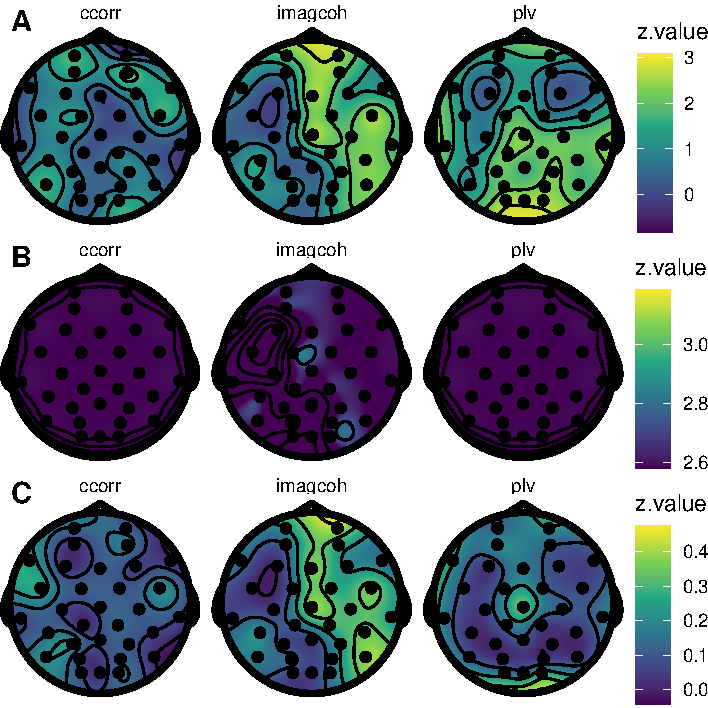
\includegraphics[width=\linewidth]{../stats/results/permutation_alpha.pdf}
  \caption{Is there an effect of the task (A, B) or the within-dyad interaction (C) on IBS in the alpha (9--14 Hz) band? After FDR correction, most values in (B) meet the significance threshold, which in that case lies at 2.58. But (B), which shuffles the spectrum instead of the original data (A), does not visualize a valid permutation test (see text). Other tests do not meet the significance threshold.}
  \label{fig:permutation_alpha}
\end{figure}

\begin{figure}[!htpb]
  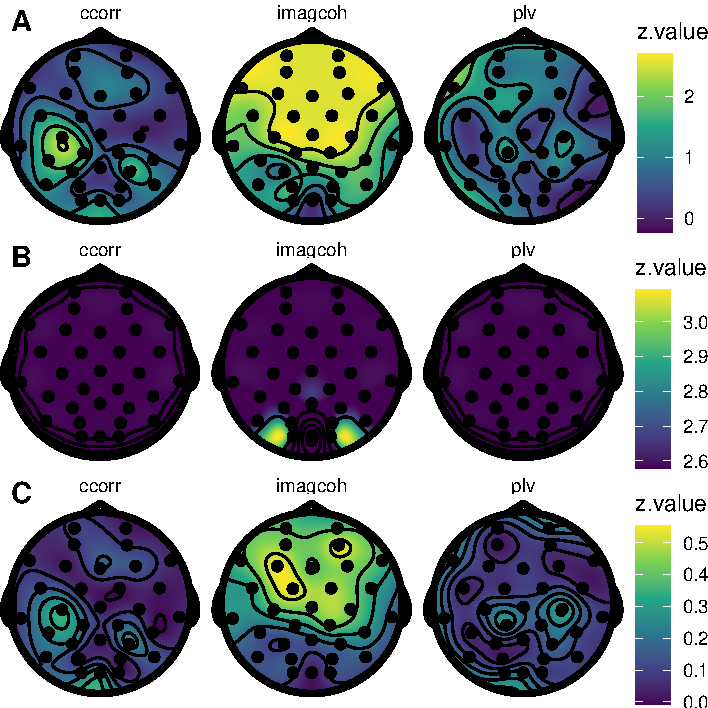
\includegraphics[width=\linewidth]{../stats/results/permutation_theta.pdf}
  \caption{Is there an effect of the task (A, B) or the within-dyad interaction (C) on IBS in the theta (4--7 Hz) band? After FDR correction, most values in (B) meet the significance threshold, which in that case lies at 2.58. But (B), which shuffles the spectrum instead of the original data (A), does not visualize a valid permutation test (see text). Other tests do not meet the significance threshold.}
  \label{fig:permutation_theta}
\end{figure}

By shuffling samples, we force the recording of one participant to be
independent from the recording of the other participant as they no longer match
up in time \parencite{lachaux_measuring_1999}. This also destroys any effects of
(temporal) task structure. There is a problem though: there are multiple ways to
shuffle samples. We can shuffle the original signal or the frequency spectrum.
If we could convert between the time and frequency domain at any resolution,
both approaches would be equivalent. But as we have previously seen in this
study, phase and amplitude information is in practice estimated over time
windows of up to a second. We run both tests to determine the differences in
practise. The permutation tests use 200 repetitions.

By shuffling dyads, we can determine whether there is something that makes the
IBS values of actual dyads different compared to randomly assembled dyads that
were never actually cooperating. As each participant saw the same stimuli in
\textcite{newman_effects_2021}'s experiment (albeit in a different order), it is
possible to construct virtual dyads such that they still saw the same stimuli.
This prevents the permutation test from detecting effects that are actually due
to the stimuli instead of the participants themselves. For this permutation
test, all possible combinations of virtual dyads are generated. As the amount of
participants is limited, this is computationally feasible.

The result of a permutation test is a large data set that has an IBS value for
each IBS measure, session, electrode, trial and permutation test repetition. We
first average out trial, then session resulting in a distribution for each
measure and electrode. Using the same averaging on the actually observed data,
we get a single value to compare each distribution against. We calculate a
p-value from this by looking how extreme this value is compared to the
distribution \parencite[see][for a robust method]{phipson_permutation_2010}.
We convert these p-values to z-scores when visualizing the results, to make any
colour transitions more gradual.

Because we perform comparisons for each measure and electrode, we control the
false discovery rate (FDR) using a \textcite{benjamini_controlling_1995}
procedure and report the resulting threshold.

\subsection{Results}

To assess whether there is an effect of the task, we perform a permutation test
where we shuffle the EEG timeseries data within trials before calculating IBS.
When we shuffle in the time domain (panel (A) in
Figures~\ref{fig:permutation_alpha}~\&~\ref{fig:permutation_theta}), we find no
significant effect. When we instead shuffle in the frequency domain, we appear
to find a significant effect almost everywhere on the scalp for all the measures
(panel (B) in Figures~\ref{fig:permutation_alpha}~\&~\ref{fig:permutation_theta}).
The only exceptions are for the imaginary part of coherency measure, which is
not significant after FDR correction for the Oz electrode in the theta band and
the F3, FC5, T7, C3, P3, Pz, O1 and Oz electrodes in the alpha band.

\begin{figure}[!htpb]
  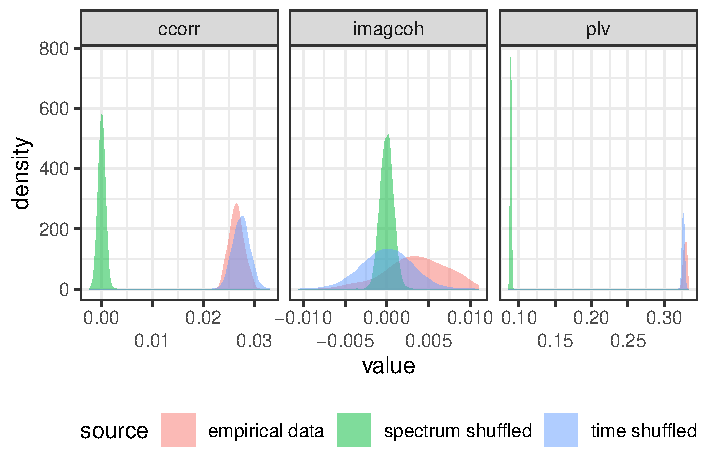
\includegraphics[width=\linewidth]{../stats/results/shuffledistributions.pdf}
  \caption{Shuffling the frequency spectrum is not equivalent to shuffling the underlying time series and then estimating the spectrum. Clearly, the shortcut of shuffling the spectrum results in a less conservative test.}
  \label{fig:shuffledistributions}
\end{figure}

\begin{figure}[!htpb]
  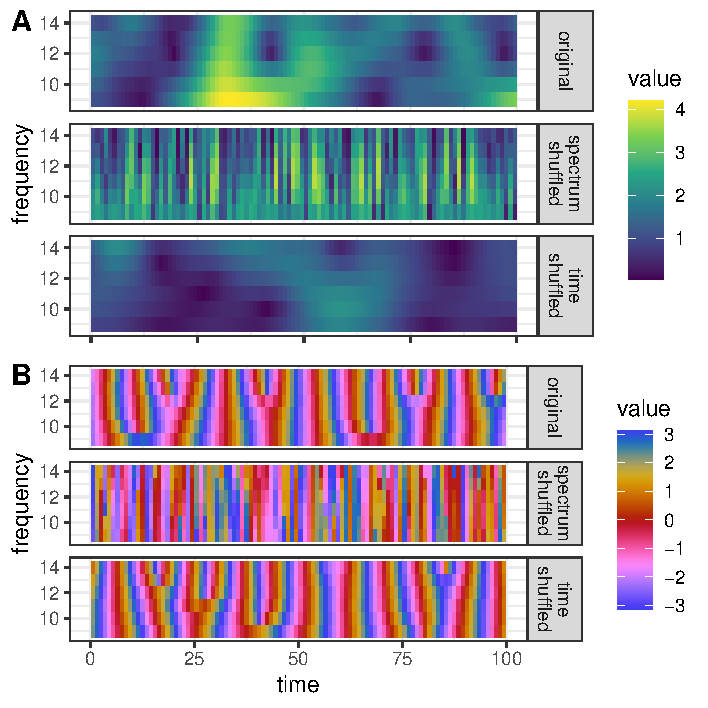
\includegraphics[width=\linewidth]{../stats/results/shufflecompare.pdf}
  \caption{An example of an original spectrum (identical to Figure~\ref{fig:freqanalysis}B \& C), the same spectrum but shuffled, and a spectrum generated from the same data but shuffled before frequency analysis. Spectrum amplitudes (A) and phases (B) are shown.}
  \label{fig:shufflecompare}
\end{figure}

Considering we could not find a task-related effect on IBS when shuffling the
time series data, it is not surprising that the tests for a within-dyad
interaction effect are also insignificant for all electrodes and measures
(panel~(C) in
Figures~\ref{fig:permutation_alpha}~\&~\ref{fig:permutation_theta}). After all,
it tests a more specific claim: whether there is an effect of working together.

\subsection{Discussion}

The difference in significance in panels (A) and (B) of
Figures~\ref{fig:permutation_alpha}~\&~\ref{fig:permutation_theta}) is because
the permutation test null distributions differ depending on the shuffling method
(see Figure~\ref{fig:shuffledistributions}). Shuffling the spectrum results in a
less conservative test. When we look at the difference between the spectra
(Figure~\ref{fig:shufflecompare}), it becomes clear that the frequency analysis
process normally results in a smoothed spectrum. But also, that this is not the
case when the spectrum is shuffled. As a result, this method of generating a
permutation test null distribution should not be used. It results in an invalid
test.

Contrary to our expectations, we found neither a task-dependent nor a
dyad-dependent effect of on IBS. As a result, testing whether this effect varies
by level of cooperation (i.e. presumably accuracy), working memory load or over
time does not make much sense. For the purpose of exploring the full IBS
pipeline, the next two sections will make an attempt regardless by analysing the
time course and trying to predict accuracy from the IBS values.

We also expected IBS in frontal and temperoparietal areas for the alpha band. No
such effect was found.

% !TEX root = thesis_draft.tex

\section{Inter-brain synchrony over time}
\label{sec:timecourse}

\begin{figure}[!htpb]
  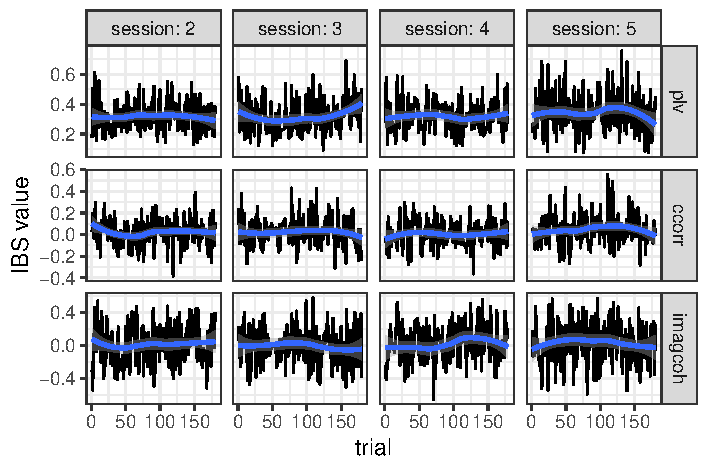
\includegraphics[width=\linewidth]{../stats/results/timecourse_repr.pdf}
  \caption{Development of inter-brain synchrony during the task. Variance is high, and there are no clear trends. (First 4 sessions only; alpha band; Pz electrode.)}
  \label{fig:timecourse_repr}
\end{figure}

\begin{figure}[!htpb]
  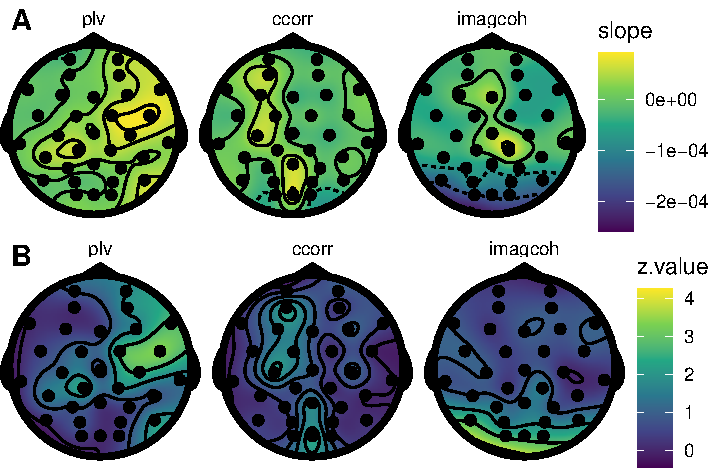
\includegraphics[width=\linewidth]{../stats/results/slopes_alpha.pdf}
  \caption{One inter-brain synchrony value is calculated per trial in the alpha band. (A) shows their (average) slope when we fit a line through them. (B) shows none of these slopes are significantly different from zero after FDR correction by comparing a linear mixed effect model that includes the slope to one that does not for each electrode.}
  \label{fig:slopes_alpha}
\end{figure}

\subsection{Introduction}

In \textcite{newman_effects_2021}'s experiment, participants need to converge on
a strategy to pick the same image or shape. As the task consists of two blocks, they
need to do so twice. We hypothesize more inter-brain synchrony (IBS) at the start of
a block, when participants need to figure out what the other is doing, and less
IBS towards the end, when participants will have switched to exploiting a by
then fixed strategy.

\subsection{Methods}

We first visualize IBS for a couple of representative sessions. Because we are
interested in effects over time that are potentially non-linear, we assess
their significance by comparing Generalized Additive Mixed Effect Models
\parencite[][GAMMs]{wood_generalized_2006} for each IBS measure. These models
contain two random effects: a factor smooth of trial by subject, and a factor
smooth of trial by electrode. This allows the model to generalize over session-
and electrode-specific trends in IBS values. GAMMs can deal with the structure
in the data caused by having multiple data points per dyad without requiring
averaging. To determine whether a given effect is significant, we add it as a
(smooth) fixed effect to one model, then compare both models.

Because it is potentially possible for effects to only show up in a couple
electrodes of interest, we additionally fit a (simpler) linear mixed effect
model with a random intercept per session on a subset of the data for each
combination of a measure and electrode. This allows us to see if there is a
linear effect of time within a session for each electrode and measure.

\subsection{Results}

Some representative timecourses of IBS data during the task are shown in
Figure~\ref{fig:timecourse_repr}. Just like with raw EEG data, there is high
variance and it can be hard to spot any trends without statistics or averaging.

No significant (smooth) effect of time (i.e. trial) was found for phase locking
value (PLV; $\chi^2(2) = 5.199, n.s.$), circular correlation
(CCorr;$\chi^2(2) = 5.862, n.s.$) or imaginary part of coherency (ImagCoh;
$\chi^2(2) = 3.734, n.s.$) in the alpha band. The same was true for the theta
band in the case of PLV ($\chi^2(2) = 4.982, n.s.$) and CCorr
($\chi^2(2) = 4.732, n.s.$), but not in the case of ImagCoh:
$\chi^2(2) = 5.805, p = 0.003$). This is due to an increase in ImagCoh values
towards the end of the second block. (A plot of the predicted values can be
found in the appendix, Figure~\ref{fig:imagcohtheta}.)

When looking at the electrode level in the alpha band, we see that the linear
effect of trial on IBS values is always close to zero
(Figure~\ref{fig:slopes_alpha}A). Unsurprisingly, none of these are
significant after FDR correction
(Figure~\ref{fig:slopes_alpha}B). It might appear as if that is not the case for
the bottom left of the ImagCoh plot, but this is an interpolation artifact:
z-values are only defined at the electrode positions. No effect of trial on IBS
was found at the electrode level in the theta band as well. (See
Figure~\ref{fig:slopes_theta} in the appendix).

\subsection{Discussion}

We found that contrary to our hypothesis, most IBS values in
\textcite{newman_effects_2021}'s experiment do not change over time, with the
possible exception of the ImagCoh values in the theta band. Interestingly, in
that case the effect was in a different direction than expected, with IBS
increasing towards the end of the block instead of going down.

One possible explanation is that performing the chosen strategy results in
similar brain activity in both participants, even if having theory of mind is
at that point no longer necessary. This could be due to performing the same
strategy, or simply due to shared environmental stimuli, like the end of the
experiment approaching. Alternatively, the assumption that towards
the end of a block participants will have converged on a strategy could be
incorrect. Finally, it is important to consider that the effect is not that big,
especially when taking into account only one out of six tests came out
significant. It could be a spurious result, especially as a robust result would
presumably be detectable by more than a single IBS measure. On the other hand,
ImagCoh is the only measure that includes amplitude information, so it could be
that it really found something the others are unable to.
\textcite{ayrolles_hypyp_2021} argue that amplitude information reflects
cognitive states better than phase information because of its larger timescale.

% !TEX root = thesis_draft.tex

\section{Prediction of task performance}

\subsection{Introduction}

We attempt to predict the performance of the dyads in
\textcite{newman_effects_2021}'s cooperation task based on inter-brain synchrony
(IBS) values and the amplitude of the P3 event-related potential (ERP)
component. There are many potential mechanisms that could cause IBS and
simultaneously be predictive of task performance. For example, functional
similarities could arise in the neural oscillations as a result of participants
placing themselves in their partner's shoes (i.e., theory of mind).
Alternatively, performing the same strategy could lead to similar brain
activity, as could focussing on the same (if chosen automatically correct)
stimulus. In the end, while the exact mechanism is interesting from a
theoretical point of view, it does not matter when the goal is to predict task
performance. Instead, it would be a possible follow-up question.

The P3 ERP component, also known as the P300 component
\parencite[p.~5]{luck_introduction_2014}, is a positive deflection in an EEG
signal about 300ms after a stimulus is shown
\parencite{sutton_evoked-potential_1965}. It generally occurs as a response to
infrequent but task-related stimuli \parencite{polich_neuropsychology_2011}.
The mechanism underlying the P3 is unclear, but the most popular theory is the
\textit{context updating model} \parencite[p.~96]{luck_introduction_2014}. It
explains the P3 as a consequence of updating the neural representation of the
environment when the stimulus (unexpectedly) changes
\parencite{polich_neuropsychology_2011}. The P3 decreases during mind-wandering
\parencite{jin_predicting_2019}. In \textcite{newman_effects_2021}'s
task the context is a bit more complex than frequent or infrequent stimuli being
shown: participants instead need to reason about how the other participant is
choosing one of the four stimuli. But this still requires keeping track of
choices, feedback and hypotheses. It is not out of the question this also
would evoke a context updating P3 ERP. Alternatively, negative feedback could be
surprising in itself when the participant believes to have hit upon a `shared
rule' on how to perform the task.

We consider a number of classification methods: logistic regression \parencite[p.137]{goodfellow_deep_2016}, support
vector machines \parencite[p.137--139]{goodfellow_deep_2016}, random decision
forests \parencite{tin_kam_ho_random_1995} and multi-layer perceptrons
\parencite{rumelhart_learning_1987}. We attempt both across-session and
within-session prediction.

\subsection{Methods}

\begin{figure}[!htpb]
  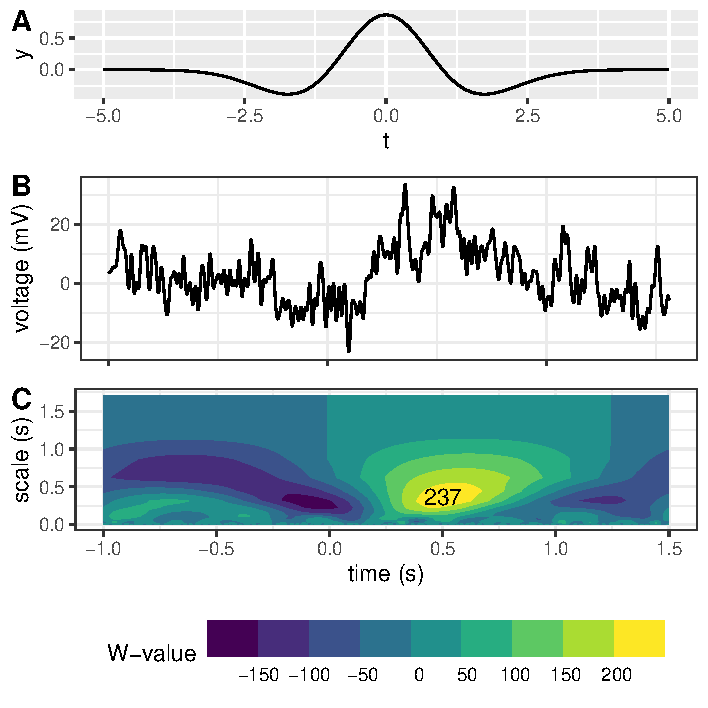
\includegraphics[width=\linewidth]{../stats/results/cwt.pdf}
  \caption{When applying the continuous wavelet transform using the mexican hat template $\psi(t)$ in (A) to an example trial $f(t)$ in (B) we obtain (C). The local maximum in (C) is shown and is our single-trial ERP measure. (B) is identical to Figure~\ref{fig:freqanalysis}A.}
  \label{fig:cwt}
\end{figure}
  
The methods of the prediction task are based on those of a study by
\textcite{jin_predicting_2019}.

Because EEG data contains a lot of noise, ERP components are normally identified
by averaging over multiple trials \parencite[p.~259]{luck_introduction_2014}.
This is not feasible when predicting task performance, as we need to predict
whether the dyad guessed correctly for each trial. Instead, we use a method that
attempts to match each trial's EEG signal with the shape of a template. The
template $\psi(t)$ takes the form of an idealized ERP component (see
Figure~\ref{fig:cwt}A). This function, sometimes called `mexican hat', is
defined as follows \parencite{bostanov_t-cwt_2006}:
\begin{equation}
\psi(t) = (1 - 16t^2)e^{-8t^2}.
\end{equation}

The method we use, which is devised by \textcite{bostanov_recognition_2004},
uses a continuous wavelet transform (CWT) to calculate the covariance between
the signal and the template at different time points and for different template
scales. The CWT is defined as \parencite{bostanov_t-cwt_2006}:
\begin{equation}
W(s, t) = \cfrac{1}{\sqrt{s}}\int\displaylimits_{-\infty}^\infty f(\tau) \cdot \psi\left(\frac{\tau - t}{s}\right) d\tau
\end{equation}
where $f(t)$ is the signal that is transformed, $s$ scales the template
$\psi(t)$ and $\tau$ shifts the template. See for an example signal
Figure~\ref{fig:cwt}B, and for a corresponding example CWT output
Figure~\ref{fig:cwt}C.

The single-trial P3 ERP is defined as the local maximum in $W(s, t)$ between
$t=250\text{ms}$ and $t=600\text{ms}$ \parencite{jin_predicting_2019}.

\begin{table}[!htbp]
\caption{Thirty sessions were randomly assigned to the train set, eight to the test set.}
\label{tab:predictionsplit}
\begin{tabularx}{\linewidth}{l X}
  \hline
  assignment & session numbers\\\hline
  train set & 2, 3, 4, 6, 8, 9, 10, 11, 12, 13, 14, 16, 18, 19, 21, 22, 23, 24, 25, 27, 29, 31, 33, 35, 36, 37, 38, 39, 41, 42\\
  test set & 5, 7, 15, 17, 20, 28, 30, 40\\\hline
\end{tabularx}
\end{table}

The data set was randomly split into a train- and a test set
(see Table~\ref{tab:predictionsplit}). The latter was not accessed during training and only used for
final model evaluation. Such a test set is sometimes also called a lock box
\parencite{hosseini_i_2020}.

Because on average dyads are correct a bit more than they are incorrect, we use
random oversampling during training to account for this imbalance in the data
set \parencite{maimon_data_2005}. Otherwise, a model that classifies every
example as correct would result in an accuracy higher than 50\%, which is not
helpful when determining whether IBS measures and the P3 component can predict
task performance.

For each trial, the three IBS measures where calculated in both the alpha and
theta band. Additionally, single-trial P3 ERP components were calculated for
both participants. These eight calculations were all repeated 32 times for each
electrode, resulting in a total of 256 features.

Phase locking value values were normalized using the inverse cumulative
density function of the normal distribution. Circular correlation and
imaginary part of coherency values were Fisher-transformed. All
single-trial ERP trials were log-transformed. This was impossible for (a trivial
amount of) negative values, which were capped at 0.05 before the transformation.
All the resulting values were additionally z-transformed.

We report sensitivity, specificity and balanced accuracy. Sensitivity looks at
correct trials. It tells us what proportion of those the classifier predicted to
be correct \parencite{yerushalmy_statistical_1947}. Specificity looks at the
incorrect trials. It tells us what proportion of those the classifier predicted
to be incorrect \parencite{yerushalmy_statistical_1947}. Balanced accuracy
is the mean of the two. Classifiers were trained to maximize balanced accuracy.

During training, 10-fold cross validation was used. Folds were chosen such that
data of a single session did not leak into both a train and validation set,
as this could potentially lead to overoptimistic accuracy estimates.

Random hyperparameter search was used \parencite{bergstra_random_2012} for 30
iterations, with hyperparameters sampled from log uniform distributions with the
exception of the random forest integer hyperparameter values, were a discrete
uniform distribution was used instead.

For the logistic regression classifier, which served as a baseline, the L1 norm
was used as it forces unused features to be dropped entirely. We optimized the
regularization strength hyperparameter $C$
\parencite[also known as \textit{capacity};][p.~117]{goodfellow_deep_2016}.

For the support vector machine, a radial basis function was used. We optimized
its radius ($\gamma$) and regularization ($C$) hyperparameters. As the SVM
performed best in earlier EEG prediction tasks
\parencite{jin_predicting_2019,lotte_review_2007}, we used it for two variations
on the experiment as well. An SVM was trained without P3 ERP component data
(i.e. taking 192 features as its input), and 256 SVMs were trained that only
took a single feature each to determine the relative importance of features. For
these variations, hyperparameter values of the main experiment were used.

Two hyperparameters were optimized for the random forest classifier. Amount of
trees (1--250) and maximum amount of features (1--30). For the multi-layer
perceptron, a fixed architecture consisting of a single hidden layer of 10
neurons was used. The ReLU function, i.e.
\begin{equation}
f(x) = \max(0, x)
\end{equation}
was used as activation function. The learning rate (alpha) was optimized.

Finally, some within-session and within-condition classification was attempted
using SVM classifiers. This results in small data sets of ~90 rows, which were
split in train sets containing ~75\% of the rows and test sets containing ~25\%.
Hyperparameter optimization was the same as in the `main' prediction experiment,
except for the choice of cross-validation folds. There were no groups to take
into account, instead folds were kept balanced such as to have both `correct'
and `incorrect' examples. A dimension reduction step using principal component
analysis (PCA) was added to better cope with the small amount of available data.
The amount of components $k$ was optimized using cross-validation.

\begin{verbatim}
\end{verbatim}

\subsection{Results}

The outcome of the cross-validation procedure used to determine the
hyperparameters was visualized in a number of parameter vs. test performance
plots. These plots can be found in Appendix~\ref{app:supplementaryfigures} for
logistic regression (Figure~\ref{fig:learning_curve_logistic}), for the SVMs
(Figure~\ref{fig:learning_curve_svm}), for the Random Forest classifier
(Figure~\ref{fig:learning_curve_rf}), for the multi-layer perceptron
(Figure~\ref{fig:learning_curve_mlp}) and finally for the within-session SVM
(Figure~\ref{fig:learning_curve_within_dyad}).

\subsubsection{Evaluation}

\begin{figure}[!htpb]
  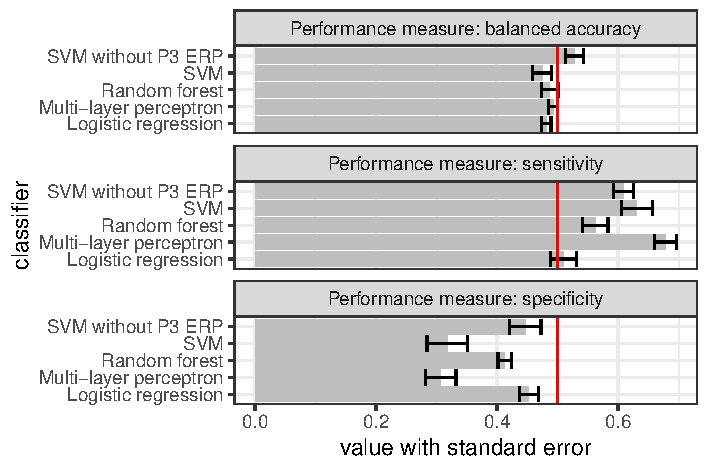
\includegraphics[width=\linewidth]{../stats/results/evaluation_avg.pdf}
  \caption{Mean classification performance on the test set for different performance metrics.}
  \label{fig:evaluation_avg}
\end{figure}

\begin{figure}[!htpb]
  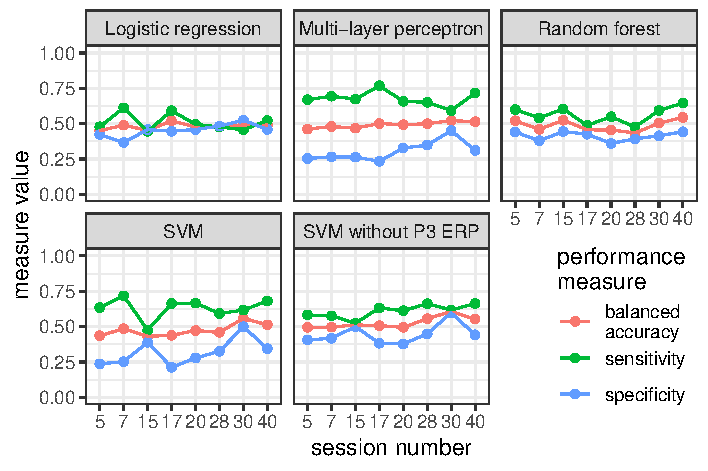
\includegraphics[width=\linewidth]{../stats/results/evaluation_detail.pdf}
  \caption{Classification performance for each test set session. (Detailed version of Figure~\ref{fig:evaluation_avg}).}
  \label{fig:evaluation_detail}
\end{figure}

Figure~\ref{fig:evaluation_avg} shows that classification performance, as
measured using the balanced accuracy, is at chance level (i.e. 0.5) for all
classifiers. Although it might seem like some error bars do not overlap with
0.5, this would be the case if confidence intervals were shown instead of
standard errors, as those are almost two times as big.
Figure~\ref{fig:evaluation_avg} also suggests that an SVM classifier that was
not trained on P3 ERP component-based features outperforms an SVM classifier
that was.

We see that all classifiers have a higher sensitivity than specificity. In other
words, the classifiers are better at predicting correct trials as correct than
incorrect trials as incorrect. This would make sense if we had not corrected for
the imbalance in the data, but between the balanced accuracy performance measure
and the random oversampling process, that is not the case. Apparently, the
classifiers converge on a (slight) bias to predict trials to be correct
regardless. This is not the case for all sessions, as can be seen in
Figure~\ref{fig:evaluation_detail}. Also, the logistic regression classifier
seems to show this phenomenon less strongly.

\subsubsection{Important features}

\begin{figure}[!htpb]
  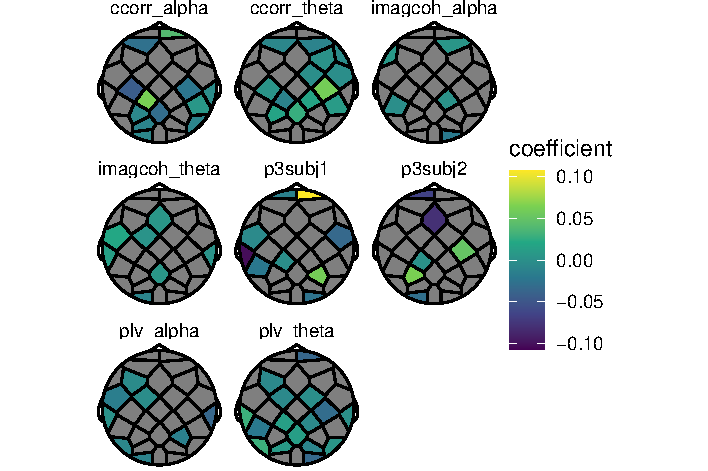
\includegraphics[width=\linewidth]{../stats/results/logistic_coef.pdf}
  \caption{Logistic regression (L1 norm): coefficients for each feature. Missing data  (grey background) means the feature was dropped by the classifier completely. Features with coefficients further from zero have a greater influence on the final prediction. Synchrony measures (ccorr = circular correlation, imagcoh = imaginary part of coherency, plv = phase locking value) were calculated for both the alpha and theta band. Both subjects contribute a P3 single-trial ERP value.}
  \label{fig:logistic_coef}
\end{figure}

The final logistic regression model drops most predictors, and puts the highest
importance on P3 ERP component features (see Figure~\ref{fig:logistic_coef}).
This is likely to be a fluke, as we would expect an actual pattern to be
duplicated among P3 ERP components for both subjects. Otherwise, no pattern is
discernible, which is what we would expect for a model that predicts at chance
level.

\begin{figure}[!htpb]
  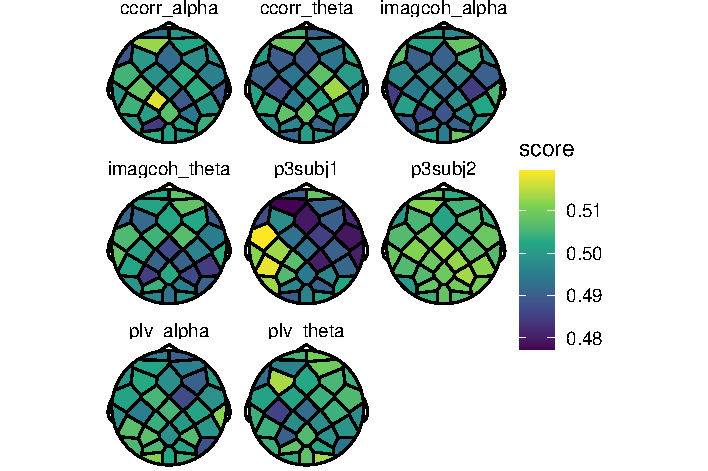
\includegraphics[width=\linewidth]{../stats/results/svm_indiv_topo.pdf}
  \caption{Balanced accuracy of SVMs trained on single features, averaged over sessions. Synchrony measures (ccorr = circular correlation, imagcoh = imaginary part of coherency, plv = phase locking value) were calculated for both the alpha and theta band. Both subjects contribute a P3 single-trial ERP value. Outliers lie further than 1.5 inter-quartile ranges from the hinge.}
  \label{fig:svm_indiv_topo}
\end{figure}

\begin{figure}[!htpb]
  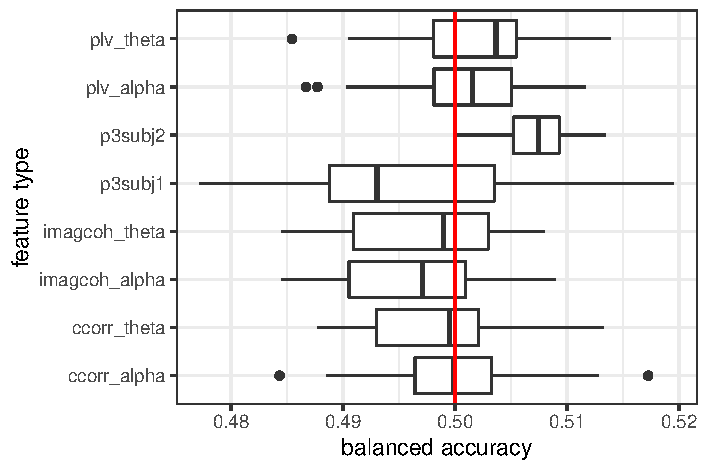
\includegraphics[width=\linewidth]{../stats/results/svm_indiv.pdf}
  \caption{Balanced accuracy of SVMs trained on single features, averaged over electrodes and sessions. A box plot summary of the data shown in Figure~\ref{fig:svm_indiv_topo}.}
  \label{fig:svm_indiv}
\end{figure}

Another way of assessing the importance of individual features in predicting
task performance is to look at the balanced accuracy of the SVMs that were
trained on single features (see Figure~\ref{fig:svm_indiv_topo}). In general,
these classifiers also perform at around chance level. There is a bit more
variation in perfomance of the classifiers that were trained on P3 ERP
components of the first participant compared to the other classifiers (see
Figure~\ref{fig:svm_indiv}). As this matches our findings using the logistic
regression classifier with L1 norm, it is likely to be caused by a pattern in
the P3 ERP component data and not just by a classifier induced artifact. But as
the pattern is again not reproduced for the second participant, it is unlikely
it contributes to predicting task performance.

\subsubsection{Within-session classification}

\begin{figure}[!htpb]
  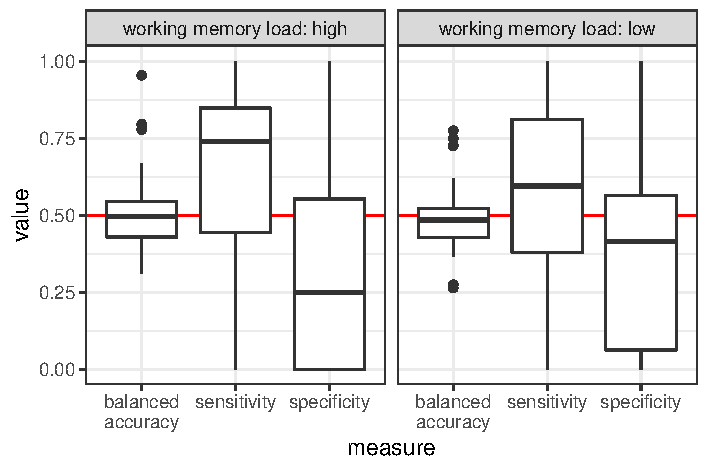
\includegraphics[width=\linewidth]{../stats/results/within_dyad_summary.pdf}
  \caption{Within-session classification performance on the test set (box plot, outliers lie further than 1.5 inter-quartile ranges from the hinge).}
  \label{fig:within_dyad_summary}
\end{figure}

\begin{figure}[!htpb]
  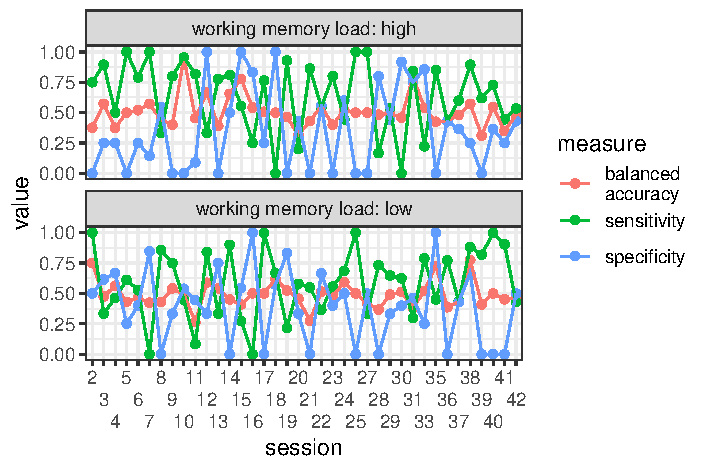
\includegraphics[width=\linewidth]{../stats/results/within_dyad_detail.pdf}
  \caption{Within-session performance on the test set (raw metrics, see Figure~\ref{fig:within_dyad_summary}) for summarized numbers.}
  \label{fig:within_dyad_detail}
\end{figure}

When predicting task performance within sessions for both low and high working
memory load, we see the same pattern as for the between-session classifiers.
Performance is still at chance level, and classifiers have on average higher
sensitivity than specificity (see Figure~\ref{fig:within_dyad_summary}).

When looking at the raw data in Figure~\ref{fig:within_dyad_detail}, we see
more variation (cf. Figure~\ref{fig:evaluation_detail}). But this is to be
expected as the test sets are much smaller.

\subsection{Discussion}

Prediction of task performance based on IBS values and single-trial
P3 ERP component values failed. There are two possible explanations for this.
It could be that another classification method would perform better. But as
different classifiers, classification scenarios and hyperparameters were tried,
another method is unlikely to yield wildly different results. The more likely
explanation is that there is simply not enough information in
IBS values and single-trial P3 ERP components to be able to predict task
performance. That would also be in line with the null results found in the time
course analysis and permutation test analysis described in this report.

While most classifiers had higher sensitivity than specificity, this was not the
case for the logistic regression classifier (see
Figure~\ref{fig:evaluation_detail}). Possibly, this is because it is one of the
more constrained models from a theoretical point of view, having a smaller
representational capacity \parencite[p.~110]{goodfellow_deep_2016}.

Interestingly, an SVM trained only on IBS values seems to perform slightly
better than one trained also on P3 ERP components. The difference is small, so
it could just be due to variation in the data. But an alternative explanation
worth considering is the \textit{curse of dimensionality}: because the data set
is relatively small compared to the amount of features, models are not
constrained all that much by the training examples
\parencite[p.~151--152]{goodfellow_deep_2016}. Leaving out features that do not
contribute much is helpful as a result. But there are other ways to constrain
classifiers. One is to force them to model the underlying distribution smoothly,
e.g. using regularization. This was the case for all discussed classifiers.
Another is to pre-process the data using a dimension reduction technique. This
approach was used for the within-session classifiers, which included a PCA step.
But that did not yield better classifiers.

The attempt to identify the most influential values in the classification
process was largely stymied by the lack of classifiers performing above chance
level. It suggests the first participant's P3 ERP component values might be more
influential. One possible explanation for that could be that the ERP component
features stand out because their distribution is the furthest from a normal
distribution. This could lead them to have an oversized effect on the models.
Negative ERP values being set to a fixed value, especially, introduces a few
(rare) outliers. Negative single-trial ERP values are rare and suggest errors in
the data cleaning, but in practise they are hard to avoid as getting rid of them
all would also throw out a lot of good data of other electrodes.

It is unlikely the first participant's P3 features are influential because they
actually help classification. In that case, we would expect them to also show up
in the P3 features for the second participant. Also, we would expect features
close to the midline to be more influential, as that is where the P3 effect is
strongest \parencite{polich_neuropsychology_2011}. Neither is the case (see
Figures~\ref{fig:logistic_coef} and~\ref{fig:svm_indiv_topo}).

Finally, a few notes. The use of balanced accuracy instead of normal accuracy is
important, as random oversampling is only used during training, not during
testing. Originally, I overlooked this, and in this case, it lead to models that
only predict a single outcome. This only became clear after looking at the
sensitivity and specificity measures. Random oversampling works well, but it can
lead to overfitting \parencite{maimon_data_2005}. Especially if the imbalance in
the data is big, it is worth considering more sophisticated methods to construct
balanced samples \parencite[][e.g. SMOTE]{maimon_data_2005}.

While performing within-session classification can profit from dyad-specific
signals that predict task performance in IBS and P3 values, it comes at a cost
of having only very little data available. In some test sets, no examples of
both correct and incorrect trials were available. This made it impossible to
train a classifier in a couple of cross-validation folds, and is also a cause of
the large variance in Figure~\ref{fig:within_dyad_detail}. The lack of data also
means that we have no choice but to randomly sample cross-validation folds from
the train set instead of respecting their causal ordering in time. When the
underlying time series is autocorrelated, as is not unlikely in EEG-derived
data, this could lead to overoptimistic predictions.

% !TEX root = thesis_draft.tex

\section{General Discussion}

We investigated the sensitivity of a hyperscanning data analysis to different
methodological choices by performing an analysis of inter-brain synchrony (IBS)
data recorded during \textcite{newman_effects_2021}'s tacit coordination task.
We built a complete analysis pipeline that tested three IBS measures: the phase
locking value (PLV), the circular correlation coefficient (CCorr) and the
imaginary part of coherency (ImagCoh). Contrary to our expectations, we found
the analysis outcome to be sensitive to relatively minor changes to this
pipeline.

All studied measures of IBS rely on a frequency analysis
step to transform the raw EEG data into the frequency domain. We found that
varying the resolution of the output or the exact tapering method used to
control spectral leakage resulted in different IBS values. The CCorr
measure was especially sensitive to such changes. As long as you are comparing
apples to apples, i.e. only values that have been calculated with the same
methodology, this variation should not be a problem. But it is a reason to
caution against comparing raw IBS values across experiments or analyses. Using
statistical methods that can take this into account, like permutation tests
that will make the same assumptions when generating a null distribution, is
recommended.

\textcite{burgess_interpretation_2013} found the CCorr measure to be less
sensitive to detecting spurious IBS than other measures. Our study did not
encounter this issue, because the permutation tests did not detect any IBS. On
the other hand, our simulation study clearly illustrates
\textcite{kayhan_deep_2022}'s observation that PLV only measures the consistency
of the phase components of the EEG signals coming from each participant, not
whether they co-vary. Most strikingly, we see it completely ignore a strong
negative linear relation between the two phase components (see
Figure~\ref{fig:simulation_local_search}). The ImagCoh measure is hardest to
evaluate. It seems to be less sensitive in general to changes in
the data it is calculated upon. For example, in the simulation study, finding
examples for different ImagCoh values was harder than for the other measures.
Also, it only responded little to changes in the frequency analysis process. If
it still picks up on `real' effects, it would be the best measure tested. But
the fact that it is so insensitive, makes me doubtful about whether it would
quantify such effects. In the end, weighing all the evidence, I would prefer
using the CCorr measure for measuring IBS. But the PLV measure is also worth
considering considering. While it has its flaws, its ubiquitousness in the
hyperscanning literature makes it more familiar to the average reader.

\subsection{Contributions}

Next to the research project's results and pipeline description, we make
available validated implementations of the PLV, CCorr and ImagCoh measures for
both MATLAB and R. During the project, we also developed a MATLAB implementation
of \textcite{mahmood_robust_2022}'s robust circular correlation measure
(Algorithm~\ref{alg:robust}), although the implementation is slow and as
discussed previously the measure itself is not well-defined from a theoretical
point of view. Finally, in the end of the simulation study section, we
describe a way to perform a power analysis for tests used in IBS studies. It
reuses the method the simulation study uses to generate fake data for a given
IBS value (Algorithm \ref{alg:optimize-measures}). As a consequence, the
test will only have access to the phase component of the signal, as the
simulation study ignored amplitude components. But that can still be useful for
power analyses of tests that target phase-based measures only.

\subsection{Limitations}

This research project, especially the simulation study part, has been heavily
focused on phase-based IBS measures. The only exception is the ImagCoh measure.
\textcite{ayrolles_hypyp_2021} suggest phase-based measures are better at
measuring ``ongoing cognitive processing'', while amplitude-based measures are
better for measuring ``cognitive state''. It would be interesting to also
consider other amplitude-based measures, like the `power envelope correlation
between orthogonalized signals' measure described by
\textcite{hipp_large-scale_2012}. That measure is also used by
\textcite{dikker_crowdsourcing_2021}, who call it `projected power correlation'
instead. Another measure that was considered for inclusion in this study is the
Kraskov mutual information measure \parencite{kraskov_estimating_2004}.
\textcite{burgess_interpretation_2013} recommends it alongside the CCorr
measure. But while \citeauthor{burgess_interpretation_2013}'s work seems to have
single-handedly popularized the latter\footnote{Most discussions of the CCorr
measure I have seen can be traced back to
\textcite{burgess_interpretation_2013}'s work
\parencite[to name just a few]{chen_trait_2021,farahzadi_towards_2021,kurihara_relationship_2022,wikstrom_inter-brain_2022,goldstein_brain--brain_2018,kingsbury_multi-brain_2020}.},
the former seems to be have much less uptake. Perhaps it is due to the lack of
implementations being available
\footnote{\url{https://github.com/otoolej/mutual_info_kNN/blob/master/mi_cont_cont.m}
comes the closest, but it is does not match
\citeauthor{burgess_interpretation_2013}'s definition exactly. For one, it does
not use an angular distance metric.}, or the more complex
(information-theoretic) definitions. At least, that is the reason why it has not
been included in the present project.

Figures~\ref{fig:permutation_alpha},~\ref{fig:permutation_theta},~\ref{fig:slopes_alpha}~and~\ref{fig:slopes_theta}
use topographical plots of the scalp that are a common sight in EEG research.
While actual values are only available for the electrode sites, the visualization
fits a surface to them to present a continuous image. While interpreting some of
these figures during this project, this lead me to the wrong conclusions at
times. For example, it is common to see extreme values around the edges of the
scalp because the surface continues on outside the data's range for a bit. As a
result, I switched to drawing Voronoi cells around the electrodes instead when
analysing the prediction data (see
Figures~\ref{fig:logistic_coef}~and~\ref{fig:svm_indiv_topo}). Of course, this
approach also has its downsides. It will be less familiar to researchers in the
field, and the discrete nature of the visualization is unrealistic.

IBS permutation tests that generate their null hypothesis distribution by
shuffling dyads, as we did in the permutation test analysis section, are a nice
way to determine whether synchrony is just task-related, or due to cooperation
within the dyad. That said, if such a test yields a significant result, there
are other possible explanations. For example, if the two participants both have
a faster response time than other dyads, this could lead to the test finding
synchrony between them that is `just' due to their early motor response. Such a
response would be solely task-related, not due to the participants working
together or interacting otherwise. It is something to keep in mind when
designing IBS experiments.

\begin{figure}[!htpb]
  \resizebox{\linewidth}{!}{% Graphic for TeX using PGF
% Title: /home/marten/AI7/MasterProject/causal.dia
% Creator: Dia v0.97.3
% CreationDate: Thu Dec 15 02:02:04 2022
% For: marten
% \usepackage{tikz}
% The following commands are not supported in PSTricks at present
% We define them conditionally, so when they are implemented,
% this pgf file will use them.
\ifx\du\undefined
  \newlength{\du}
\fi
\setlength{\du}{15\unitlength}
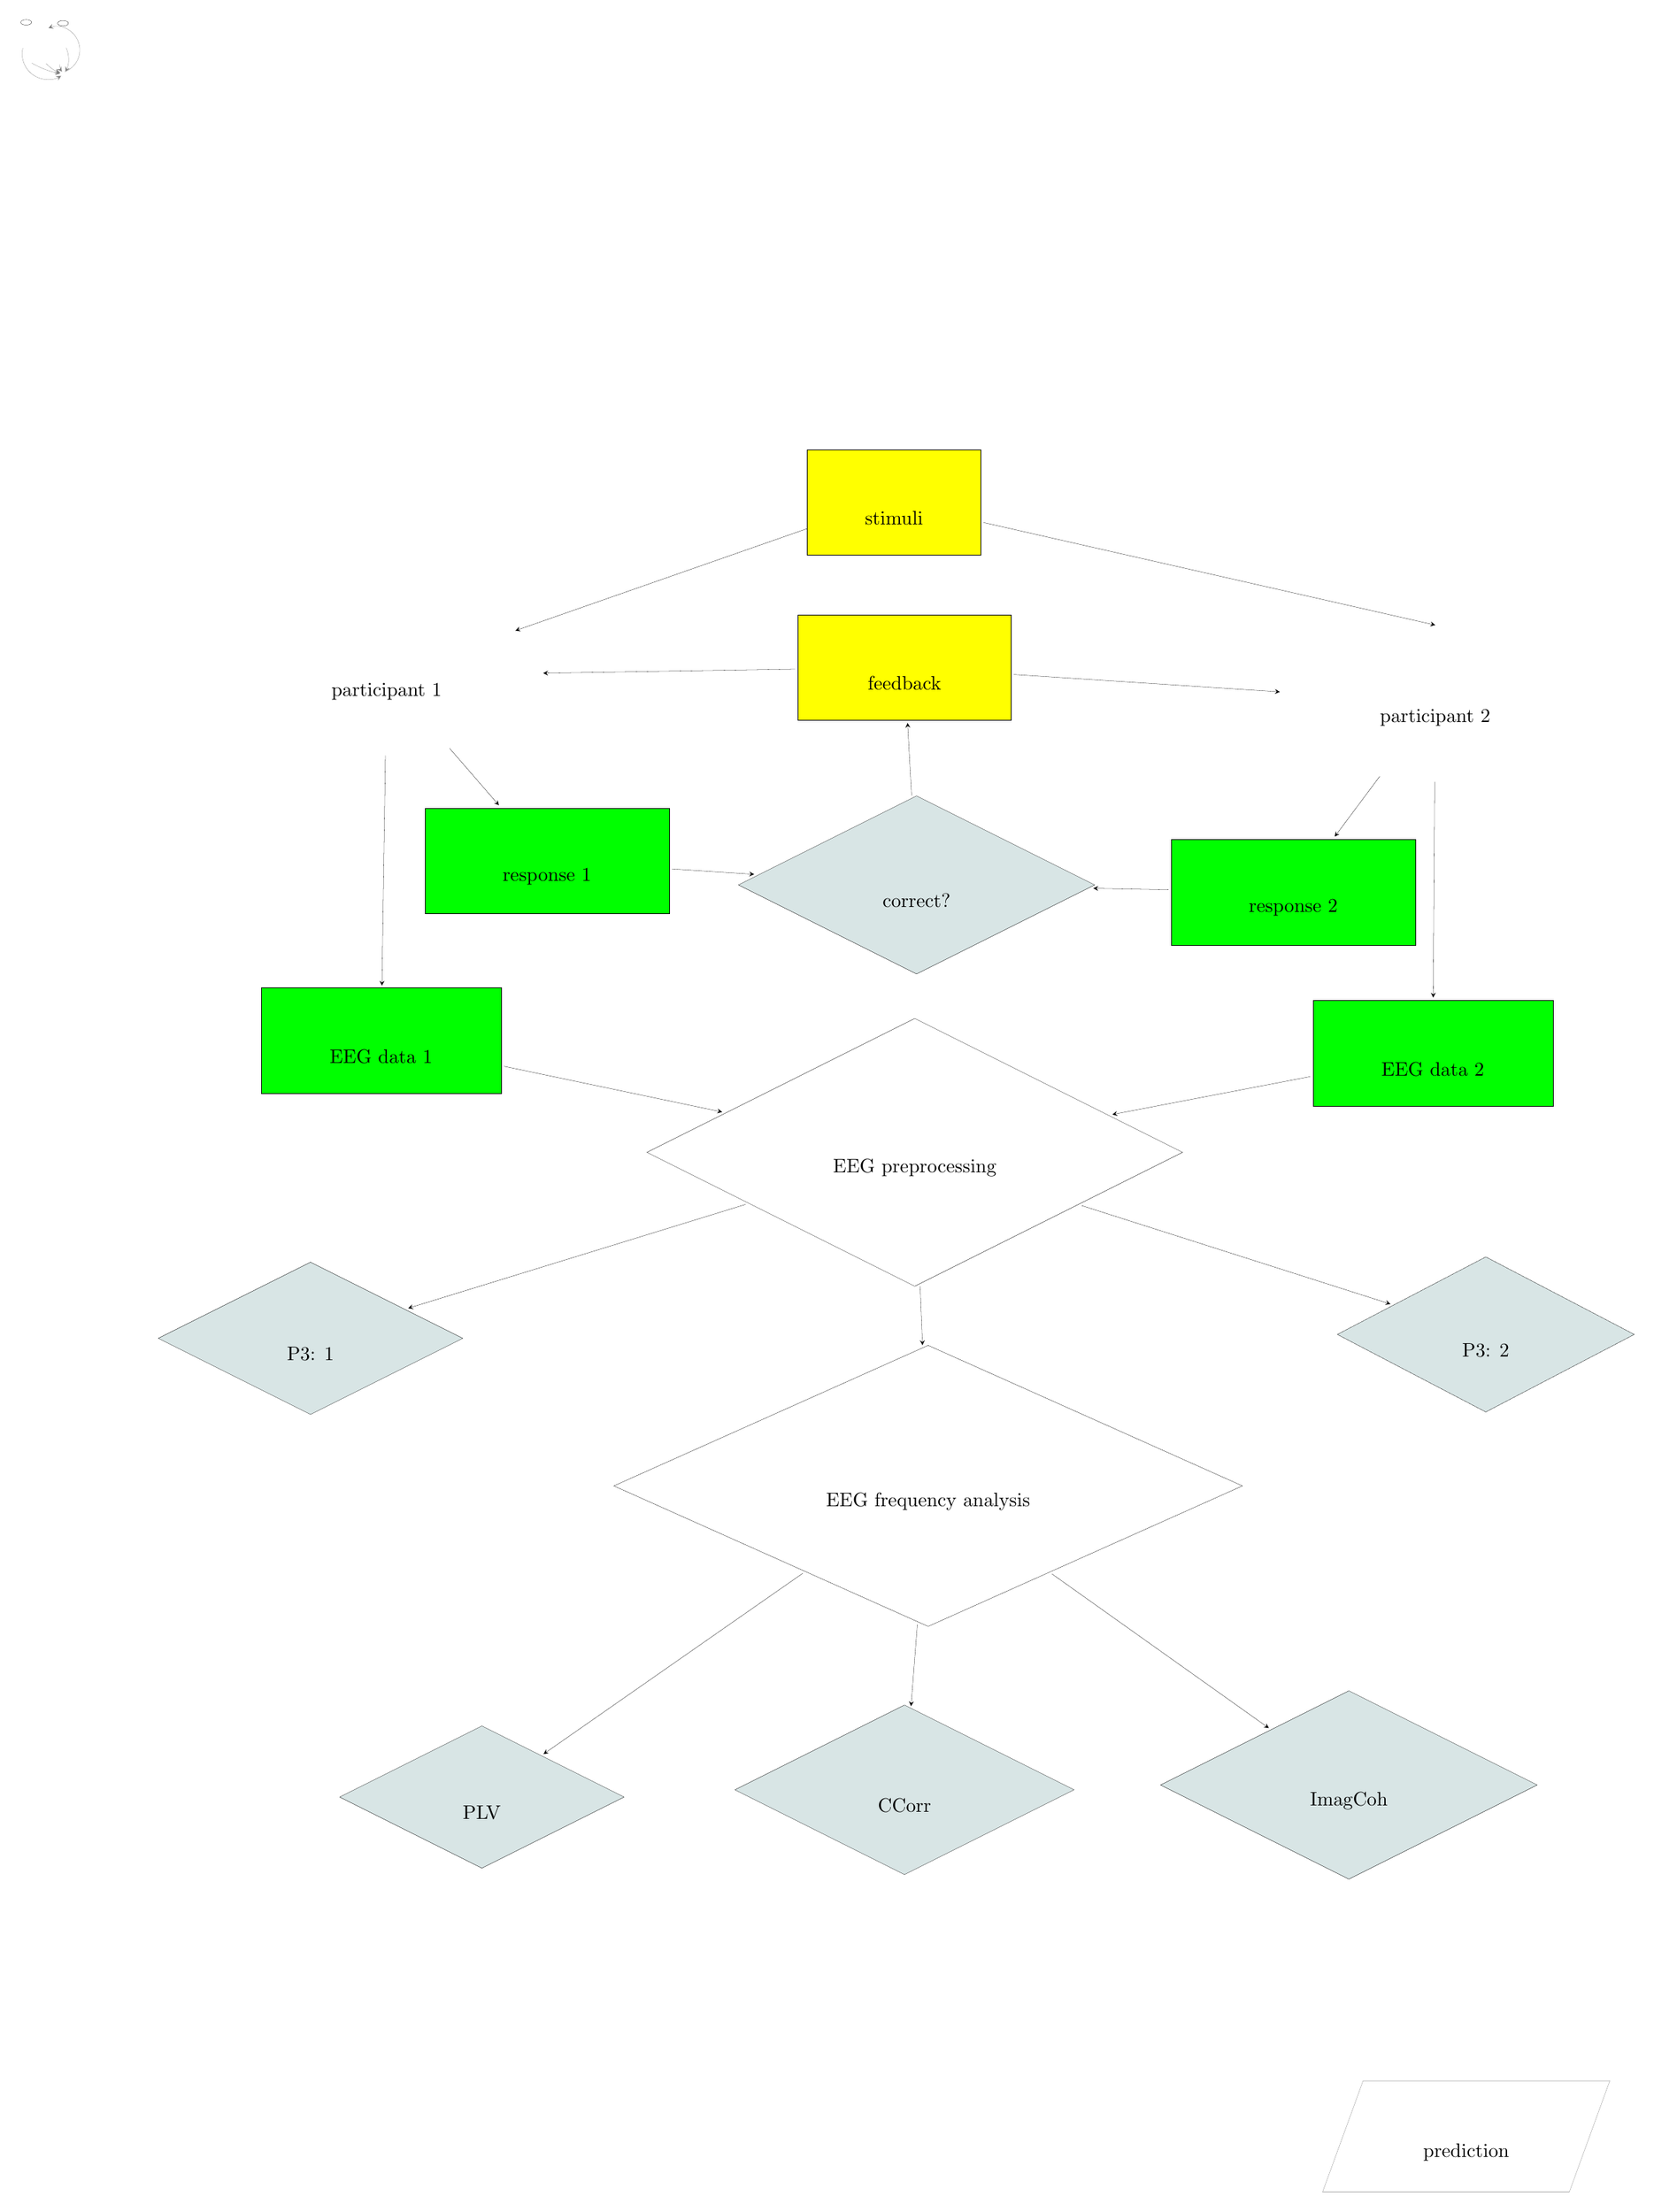
\begin{tikzpicture}
\pgftransformxscale{1.000000}
\pgftransformyscale{-1.000000}
\definecolor{dialinecolor}{rgb}{0.000000, 0.000000, 0.000000}
\pgfsetstrokecolor{dialinecolor}
\definecolor{dialinecolor}{rgb}{1.000000, 1.000000, 1.000000}
\pgfsetfillcolor{dialinecolor}
\definecolor{dialinecolor}{rgb}{1.000000, 1.000000, 1.000000}
\pgfsetfillcolor{dialinecolor}
\fill (24.287240\du,37.467200\du)--(28.725917\du,37.467200\du)--(27.997976\du,39.467200\du)--(23.559300\du,39.467200\du)--cycle;
\pgfsetlinewidth{0.100000\du}
\pgfsetdash{}{0pt}
\pgfsetdash{}{0pt}
\pgfsetmiterjoin
\definecolor{dialinecolor}{rgb}{0.498039, 0.498039, 0.498039}
\pgfsetstrokecolor{dialinecolor}
\draw (24.287240\du,37.467200\du)--(28.725917\du,37.467200\du)--(27.997976\du,39.467200\du)--(23.559300\du,39.467200\du)--cycle;
% setfont left to latex
\definecolor{dialinecolor}{rgb}{0.000000, 0.000000, 0.000000}
\pgfsetstrokecolor{dialinecolor}
\node at (26.142608\du,38.751360\du){prediction};
\pgfsetlinewidth{0.100000\du}
\pgfsetdash{}{0pt}
\pgfsetdash{}{0pt}
\pgfsetbuttcap
{
\definecolor{dialinecolor}{rgb}{0.498039, 0.498039, 0.498039}
\pgfsetfillcolor{dialinecolor}
% was here!!!
\pgfsetarrowsend{stealth}
\definecolor{dialinecolor}{rgb}{0.498039, 0.498039, 0.498039}
\pgfsetstrokecolor{dialinecolor}
\pgfpathmoveto{\pgfpoint{5.004066\du}{25.350989\du}}
\pgfpatharc{193}{59}{13.157261\du and 13.157261\du}
\pgfusepath{stroke}
}
\pgfsetlinewidth{0.100000\du}
\pgfsetdash{}{0pt}
\pgfsetdash{}{0pt}
\pgfsetbuttcap
{
\definecolor{dialinecolor}{rgb}{0.498039, 0.498039, 0.498039}
\pgfsetfillcolor{dialinecolor}
% was here!!!
\pgfsetarrowsend{stealth}
\definecolor{dialinecolor}{rgb}{0.498039, 0.498039, 0.498039}
\pgfsetstrokecolor{dialinecolor}
\pgfpathmoveto{\pgfpoint{9.657185\du}{33.076071\du}}
\pgfpatharc{120}{100}{44.359140\du and 44.359140\du}
\pgfusepath{stroke}
}
\pgfsetlinewidth{0.100000\du}
\pgfsetdash{}{0pt}
\pgfsetdash{}{0pt}
\pgfsetbuttcap
{
\definecolor{dialinecolor}{rgb}{0.498039, 0.498039, 0.498039}
\pgfsetfillcolor{dialinecolor}
% was here!!!
\pgfsetarrowsend{stealth}
\definecolor{dialinecolor}{rgb}{0.498039, 0.498039, 0.498039}
\pgfsetstrokecolor{dialinecolor}
\pgfpathmoveto{\pgfpoint{17.001187\du}{33.320496\du}}
\pgfpatharc{137}{110}{18.125522\du and 18.125522\du}
\pgfusepath{stroke}
}
\pgfsetlinewidth{0.100000\du}
\pgfsetdash{}{0pt}
\pgfsetdash{}{0pt}
\pgfsetbuttcap
{
\definecolor{dialinecolor}{rgb}{0.498039, 0.498039, 0.498039}
\pgfsetfillcolor{dialinecolor}
% was here!!!
\pgfsetarrowsend{stealth}
\definecolor{dialinecolor}{rgb}{0.498039, 0.498039, 0.498039}
\pgfsetstrokecolor{dialinecolor}
\pgfpathmoveto{\pgfpoint{23.827651\du}{33.786128\du}}
\pgfpatharc{180}{143}{6.054480\du and 6.054480\du}
\pgfusepath{stroke}
}
\pgfsetlinewidth{0.100000\du}
\pgfsetdash{}{0pt}
\pgfsetdash{}{0pt}
\pgfsetbuttcap
{
\definecolor{dialinecolor}{rgb}{0.498039, 0.498039, 0.498039}
\pgfsetfillcolor{dialinecolor}
% was here!!!
\pgfsetarrowsend{stealth}
\definecolor{dialinecolor}{rgb}{0.498039, 0.498039, 0.498039}
\pgfsetstrokecolor{dialinecolor}
\pgfpathmoveto{\pgfpoint{26.505631\du}{37.467573\du}}
\pgfpatharc{69}{-110}{11.947093\du and 11.947093\du}
\pgfusepath{stroke}
}
\definecolor{dialinecolor}{rgb}{1.000000, 1.000000, 0.000000}
\pgfsetfillcolor{dialinecolor}
\fill (14.286900\du,8.112710\du)--(14.286900\du,10.012710\du)--(17.411900\du,10.012710\du)--(17.411900\du,8.112710\du)--cycle;
\pgfsetlinewidth{0.100000\du}
\pgfsetdash{}{0pt}
\pgfsetdash{}{0pt}
\pgfsetmiterjoin
\definecolor{dialinecolor}{rgb}{0.000000, 0.000000, 0.000000}
\pgfsetstrokecolor{dialinecolor}
\draw (14.286900\du,8.112710\du)--(14.286900\du,10.012710\du)--(17.411900\du,10.012710\du)--(17.411900\du,8.112710\du)--cycle;
% setfont left to latex
\definecolor{dialinecolor}{rgb}{0.000000, 0.000000, 0.000000}
\pgfsetstrokecolor{dialinecolor}
\node at (15.849400\du,9.346870\du){stimuli};
\definecolor{dialinecolor}{rgb}{1.000000, 1.000000, 0.000000}
\pgfsetfillcolor{dialinecolor}
\fill (14.119700\du,11.084400\du)--(14.119700\du,12.984400\du)--(17.954700\du,12.984400\du)--(17.954700\du,11.084400\du)--cycle;
\pgfsetlinewidth{0.100000\du}
\pgfsetdash{}{0pt}
\pgfsetdash{}{0pt}
\pgfsetmiterjoin
\definecolor{dialinecolor}{rgb}{0.000000, 0.000000, 0.000000}
\pgfsetstrokecolor{dialinecolor}
\draw (14.119700\du,11.084400\du)--(14.119700\du,12.984400\du)--(17.954700\du,12.984400\du)--(17.954700\du,11.084400\du)--cycle;
% setfont left to latex
\definecolor{dialinecolor}{rgb}{0.000000, 0.000000, 0.000000}
\pgfsetstrokecolor{dialinecolor}
\node at (16.037200\du,12.318560\du){feedback};
\definecolor{dialinecolor}{rgb}{1.000000, 1.000000, 1.000000}
\pgfsetfillcolor{dialinecolor}
\pgfpathellipse{\pgfpoint{6.720752\du}{12.183961\du}}{\pgfpoint{2.769322\du}{0\du}}{\pgfpoint{0\du}{1.384661\du}}
\pgfusepath{fill}
\pgfsetlinewidth{0.100000\du}
\pgfsetdash{}{0pt}
\pgfsetdash{}{0pt}
\pgfsetmiterjoin
\definecolor{dialinecolor}{rgb}{0.000000, 0.000000, 0.000000}
\pgfsetstrokecolor{dialinecolor}
\pgfpathellipse{\pgfpoint{6.720752\du}{12.183961\du}}{\pgfpoint{2.769322\du}{0\du}}{\pgfpoint{0\du}{1.384661\du}}
\pgfusepath{stroke}
% setfont left to latex
\definecolor{dialinecolor}{rgb}{0.000000, 0.000000, 0.000000}
\pgfsetstrokecolor{dialinecolor}
\node at (6.720752\du,12.468121\du){participant 1};
\definecolor{dialinecolor}{rgb}{1.000000, 1.000000, 1.000000}
\pgfsetfillcolor{dialinecolor}
\pgfpathellipse{\pgfpoint{25.584822\du}{12.657761\du}}{\pgfpoint{2.769322\du}{0\du}}{\pgfpoint{0\du}{1.384661\du}}
\pgfusepath{fill}
\pgfsetlinewidth{0.100000\du}
\pgfsetdash{}{0pt}
\pgfsetdash{}{0pt}
\pgfsetmiterjoin
\definecolor{dialinecolor}{rgb}{0.000000, 0.000000, 0.000000}
\pgfsetstrokecolor{dialinecolor}
\pgfpathellipse{\pgfpoint{25.584822\du}{12.657761\du}}{\pgfpoint{2.769322\du}{0\du}}{\pgfpoint{0\du}{1.384661\du}}
\pgfusepath{stroke}
% setfont left to latex
\definecolor{dialinecolor}{rgb}{0.000000, 0.000000, 0.000000}
\pgfsetstrokecolor{dialinecolor}
\node at (25.584822\du,12.941921\du){participant 2};
\pgfsetlinewidth{0.100000\du}
\pgfsetdash{}{0pt}
\pgfsetdash{}{0pt}
\pgfsetbuttcap
{
\definecolor{dialinecolor}{rgb}{0.000000, 0.000000, 0.000000}
\pgfsetfillcolor{dialinecolor}
% was here!!!
\pgfsetarrowsend{stealth}
\definecolor{dialinecolor}{rgb}{0.000000, 0.000000, 0.000000}
\pgfsetstrokecolor{dialinecolor}
\draw (14.286900\du,9.537710\du)--(9.037608\du,11.373644\du);
}
\pgfsetlinewidth{0.100000\du}
\pgfsetdash{}{0pt}
\pgfsetdash{}{0pt}
\pgfsetbuttcap
{
\definecolor{dialinecolor}{rgb}{0.000000, 0.000000, 0.000000}
\pgfsetfillcolor{dialinecolor}
% was here!!!
\pgfsetarrowsend{stealth}
\definecolor{dialinecolor}{rgb}{0.000000, 0.000000, 0.000000}
\pgfsetstrokecolor{dialinecolor}
\draw (17.461469\du,9.428725\du)--(25.584800\du,11.273100\du);
}
\pgfsetlinewidth{0.100000\du}
\pgfsetdash{}{0pt}
\pgfsetdash{}{0pt}
\pgfsetbuttcap
{
\definecolor{dialinecolor}{rgb}{0.000000, 0.000000, 0.000000}
\pgfsetfillcolor{dialinecolor}
% was here!!!
\pgfsetarrowsend{stealth}
\definecolor{dialinecolor}{rgb}{0.000000, 0.000000, 0.000000}
\pgfsetstrokecolor{dialinecolor}
\draw (14.069453\du,12.065989\du)--(9.537749\du,12.138739\du);
}
\pgfsetlinewidth{0.100000\du}
\pgfsetdash{}{0pt}
\pgfsetdash{}{0pt}
\pgfsetbuttcap
{
\definecolor{dialinecolor}{rgb}{0.000000, 0.000000, 0.000000}
\pgfsetfillcolor{dialinecolor}
% was here!!!
\pgfsetarrowsend{stealth}
\definecolor{dialinecolor}{rgb}{0.000000, 0.000000, 0.000000}
\pgfsetstrokecolor{dialinecolor}
\draw (18.005115\du,12.162885\du)--(22.789415\du,12.475250\du);
}
\definecolor{dialinecolor}{rgb}{0.000000, 1.000000, 0.000000}
\pgfsetfillcolor{dialinecolor}
\fill (7.409660\du,14.564600\du)--(7.409660\du,16.464600\du)--(11.804660\du,16.464600\du)--(11.804660\du,14.564600\du)--cycle;
\pgfsetlinewidth{0.100000\du}
\pgfsetdash{}{0pt}
\pgfsetdash{}{0pt}
\pgfsetmiterjoin
\definecolor{dialinecolor}{rgb}{0.000000, 0.000000, 0.000000}
\pgfsetstrokecolor{dialinecolor}
\draw (7.409660\du,14.564600\du)--(7.409660\du,16.464600\du)--(11.804660\du,16.464600\du)--(11.804660\du,14.564600\du)--cycle;
% setfont left to latex
\definecolor{dialinecolor}{rgb}{0.000000, 0.000000, 0.000000}
\pgfsetstrokecolor{dialinecolor}
\node at (9.607160\du,15.798760\du){response 1};
\definecolor{dialinecolor}{rgb}{0.000000, 1.000000, 0.000000}
\pgfsetfillcolor{dialinecolor}
\fill (20.835000\du,15.129400\du)--(20.835000\du,17.029400\du)--(25.230000\du,17.029400\du)--(25.230000\du,15.129400\du)--cycle;
\pgfsetlinewidth{0.100000\du}
\pgfsetdash{}{0pt}
\pgfsetdash{}{0pt}
\pgfsetmiterjoin
\definecolor{dialinecolor}{rgb}{0.000000, 0.000000, 0.000000}
\pgfsetstrokecolor{dialinecolor}
\draw (20.835000\du,15.129400\du)--(20.835000\du,17.029400\du)--(25.230000\du,17.029400\du)--(25.230000\du,15.129400\du)--cycle;
% setfont left to latex
\definecolor{dialinecolor}{rgb}{0.000000, 0.000000, 0.000000}
\pgfsetstrokecolor{dialinecolor}
\node at (23.032500\du,16.363560\du){response 2};
\pgfsetlinewidth{0.100000\du}
\pgfsetdash{}{0pt}
\pgfsetdash{}{0pt}
\pgfsetbuttcap
{
\definecolor{dialinecolor}{rgb}{0.000000, 0.000000, 0.000000}
\pgfsetfillcolor{dialinecolor}
% was here!!!
\pgfsetarrowsend{stealth}
\definecolor{dialinecolor}{rgb}{0.000000, 0.000000, 0.000000}
\pgfsetstrokecolor{dialinecolor}
\draw (7.854245\du,13.491904\du)--(8.741097\du,14.515246\du);
}
\pgfsetlinewidth{0.100000\du}
\pgfsetdash{}{0pt}
\pgfsetdash{}{0pt}
\pgfsetbuttcap
{
\definecolor{dialinecolor}{rgb}{0.000000, 0.000000, 0.000000}
\pgfsetfillcolor{dialinecolor}
% was here!!!
\pgfsetarrowsend{stealth}
\definecolor{dialinecolor}{rgb}{0.000000, 0.000000, 0.000000}
\pgfsetstrokecolor{dialinecolor}
\draw (24.587042\du,13.995383\du)--(23.778381\du,15.079473\du);
}
\definecolor{dialinecolor}{rgb}{0.847059, 0.898039, 0.898039}
\pgfsetfillcolor{dialinecolor}
\fill (16.254610\du,14.346800\du)--(19.459020\du,15.949005\du)--(16.254610\du,17.551210\du)--(13.050200\du,15.949005\du)--cycle;
\pgfsetlinewidth{0.100000\du}
\pgfsetdash{}{0pt}
\pgfsetdash{}{0pt}
\pgfsetmiterjoin
\definecolor{dialinecolor}{rgb}{0.000000, 0.000000, 0.000000}
\pgfsetstrokecolor{dialinecolor}
\draw (16.254610\du,14.346800\du)--(19.459020\du,15.949005\du)--(16.254610\du,17.551210\du)--(13.050200\du,15.949005\du)--cycle;
% setfont left to latex
\definecolor{dialinecolor}{rgb}{0.000000, 0.000000, 0.000000}
\pgfsetstrokecolor{dialinecolor}
\node at (16.254610\du,16.233165\du){correct?};
\pgfsetlinewidth{0.100000\du}
\pgfsetdash{}{0pt}
\pgfsetdash{}{0pt}
\pgfsetbuttcap
{
\definecolor{dialinecolor}{rgb}{0.000000, 0.000000, 0.000000}
\pgfsetfillcolor{dialinecolor}
% was here!!!
\pgfsetarrowsend{stealth}
\definecolor{dialinecolor}{rgb}{0.000000, 0.000000, 0.000000}
\pgfsetstrokecolor{dialinecolor}
\draw (11.854083\du,15.661434\du)--(13.332556\du,15.758051\du);
}
\pgfsetlinewidth{0.100000\du}
\pgfsetdash{}{0pt}
\pgfsetdash{}{0pt}
\pgfsetbuttcap
{
\definecolor{dialinecolor}{rgb}{0.000000, 0.000000, 0.000000}
\pgfsetfillcolor{dialinecolor}
% was here!!!
\pgfsetarrowsend{stealth}
\definecolor{dialinecolor}{rgb}{0.000000, 0.000000, 0.000000}
\pgfsetstrokecolor{dialinecolor}
\draw (20.784925\du,16.036161\du)--(19.435056\du,16.010191\du);
}
\pgfsetlinewidth{0.100000\du}
\pgfsetdash{}{0pt}
\pgfsetdash{}{0pt}
\pgfsetbuttcap
{
\definecolor{dialinecolor}{rgb}{0.000000, 0.000000, 0.000000}
\pgfsetfillcolor{dialinecolor}
% was here!!!
\pgfsetarrowsend{stealth}
\definecolor{dialinecolor}{rgb}{0.000000, 0.000000, 0.000000}
\pgfsetstrokecolor{dialinecolor}
\draw (16.165305\du,14.341016\du)--(16.092747\du,13.034555\du);
}
\pgfsetlinewidth{0.100000\du}
\pgfsetdash{}{0pt}
\pgfsetdash{}{0pt}
\pgfsetbuttcap
{
\definecolor{dialinecolor}{rgb}{0.000000, 0.000000, 0.000000}
\pgfsetfillcolor{dialinecolor}
% was here!!!
\pgfsetarrowsend{stealth}
\definecolor{dialinecolor}{rgb}{0.000000, 0.000000, 0.000000}
\pgfsetstrokecolor{dialinecolor}
\draw (6.699028\du,13.618905\du)--(6.636308\du,17.761850\du);
}
\pgfsetlinewidth{0.100000\du}
\pgfsetdash{}{0pt}
\pgfsetdash{}{0pt}
\pgfsetbuttcap
{
\definecolor{dialinecolor}{rgb}{0.000000, 0.000000, 0.000000}
\pgfsetfillcolor{dialinecolor}
% was here!!!
\pgfsetarrowsend{stealth}
\definecolor{dialinecolor}{rgb}{0.000000, 0.000000, 0.000000}
\pgfsetstrokecolor{dialinecolor}
\draw (25.575267\du,14.092571\du)--(25.549409\du,17.975544\du);
}
\definecolor{dialinecolor}{rgb}{0.000000, 1.000000, 0.000000}
\pgfsetfillcolor{dialinecolor}
\fill (4.462610\du,17.799200\du)--(4.462610\du,19.699200\du)--(8.780110\du,19.699200\du)--(8.780110\du,17.799200\du)--cycle;
\pgfsetlinewidth{0.100000\du}
\pgfsetdash{}{0pt}
\pgfsetdash{}{0pt}
\pgfsetmiterjoin
\definecolor{dialinecolor}{rgb}{0.000000, 0.000000, 0.000000}
\pgfsetstrokecolor{dialinecolor}
\draw (4.462610\du,17.799200\du)--(4.462610\du,19.699200\du)--(8.780110\du,19.699200\du)--(8.780110\du,17.799200\du)--cycle;
% setfont left to latex
\definecolor{dialinecolor}{rgb}{0.000000, 0.000000, 0.000000}
\pgfsetstrokecolor{dialinecolor}
\node at (6.621360\du,19.033360\du){EEG data 1};
\definecolor{dialinecolor}{rgb}{0.000000, 1.000000, 0.000000}
\pgfsetfillcolor{dialinecolor}
\fill (23.384000\du,18.025400\du)--(23.384000\du,19.925400\du)--(27.701500\du,19.925400\du)--(27.701500\du,18.025400\du)--cycle;
\pgfsetlinewidth{0.100000\du}
\pgfsetdash{}{0pt}
\pgfsetdash{}{0pt}
\pgfsetmiterjoin
\definecolor{dialinecolor}{rgb}{0.000000, 0.000000, 0.000000}
\pgfsetstrokecolor{dialinecolor}
\draw (23.384000\du,18.025400\du)--(23.384000\du,19.925400\du)--(27.701500\du,19.925400\du)--(27.701500\du,18.025400\du)--cycle;
% setfont left to latex
\definecolor{dialinecolor}{rgb}{0.000000, 0.000000, 0.000000}
\pgfsetstrokecolor{dialinecolor}
\node at (25.542750\du,19.259560\du){EEG data 2};
\definecolor{dialinecolor}{rgb}{1.000000, 1.000000, 1.000000}
\pgfsetfillcolor{dialinecolor}
\fill (16.462669\du,24.234300\du)--(22.117037\du,26.762637\du)--(16.462669\du,29.290975\du)--(10.808300\du,26.762637\du)--cycle;
\pgfsetlinewidth{0.100000\du}
\pgfsetdash{}{0pt}
\pgfsetdash{}{0pt}
\pgfsetmiterjoin
\definecolor{dialinecolor}{rgb}{0.000000, 0.000000, 0.000000}
\pgfsetstrokecolor{dialinecolor}
\draw (16.462669\du,24.234300\du)--(22.117037\du,26.762637\du)--(16.462669\du,29.290975\du)--(10.808300\du,26.762637\du)--cycle;
% setfont left to latex
\definecolor{dialinecolor}{rgb}{0.000000, 0.000000, 0.000000}
\pgfsetstrokecolor{dialinecolor}
\node at (16.462669\du,27.046798\du){EEG frequency analysis};
\definecolor{dialinecolor}{rgb}{0.847059, 0.898039, 0.898039}
\pgfsetfillcolor{dialinecolor}
\fill (8.434070\du,31.082300\du)--(10.992230\du,32.361380\du)--(8.434070\du,33.640460\du)--(5.875910\du,32.361380\du)--cycle;
\pgfsetlinewidth{0.100000\du}
\pgfsetdash{}{0pt}
\pgfsetdash{}{0pt}
\pgfsetmiterjoin
\definecolor{dialinecolor}{rgb}{0.000000, 0.000000, 0.000000}
\pgfsetstrokecolor{dialinecolor}
\draw (8.434070\du,31.082300\du)--(10.992230\du,32.361380\du)--(8.434070\du,33.640460\du)--(5.875910\du,32.361380\du)--cycle;
% setfont left to latex
\definecolor{dialinecolor}{rgb}{0.000000, 0.000000, 0.000000}
\pgfsetstrokecolor{dialinecolor}
\node at (8.434070\du,32.645540\du){PLV};
\pgfsetlinewidth{0.100000\du}
\pgfsetdash{}{0pt}
\pgfsetdash{}{0pt}
\pgfsetbuttcap
{
\definecolor{dialinecolor}{rgb}{0.000000, 0.000000, 0.000000}
\pgfsetfillcolor{dialinecolor}
% was here!!!
\pgfsetarrowsend{stealth}
\definecolor{dialinecolor}{rgb}{0.000000, 0.000000, 0.000000}
\pgfsetstrokecolor{dialinecolor}
\draw (14.210016\du,28.333525\du)--(9.543981\du,31.587384\du);
}
\definecolor{dialinecolor}{rgb}{0.847059, 0.898039, 0.898039}
\pgfsetfillcolor{dialinecolor}
\fill (16.037460\du,30.705700\du)--(19.088120\du,32.231030\du)--(16.037460\du,33.756360\du)--(12.986800\du,32.231030\du)--cycle;
\pgfsetlinewidth{0.100000\du}
\pgfsetdash{}{0pt}
\pgfsetdash{}{0pt}
\pgfsetmiterjoin
\definecolor{dialinecolor}{rgb}{0.000000, 0.000000, 0.000000}
\pgfsetstrokecolor{dialinecolor}
\draw (16.037460\du,30.705700\du)--(19.088120\du,32.231030\du)--(16.037460\du,33.756360\du)--(12.986800\du,32.231030\du)--cycle;
% setfont left to latex
\definecolor{dialinecolor}{rgb}{0.000000, 0.000000, 0.000000}
\pgfsetstrokecolor{dialinecolor}
\node at (16.037460\du,32.515190\du){CCorr};
\pgfsetlinewidth{0.100000\du}
\pgfsetdash{}{0pt}
\pgfsetdash{}{0pt}
\pgfsetbuttcap
{
\definecolor{dialinecolor}{rgb}{0.000000, 0.000000, 0.000000}
\pgfsetfillcolor{dialinecolor}
% was here!!!
\pgfsetarrowsend{stealth}
\definecolor{dialinecolor}{rgb}{0.000000, 0.000000, 0.000000}
\pgfsetstrokecolor{dialinecolor}
\draw (16.268906\du,29.254521\du)--(16.154559\du,30.725086\du);
}
\definecolor{dialinecolor}{rgb}{0.847059, 0.898039, 0.898039}
\pgfsetfillcolor{dialinecolor}
\fill (24.031760\du,30.450100\du)--(27.419920\du,32.144180\du)--(24.031760\du,33.838260\du)--(20.643600\du,32.144180\du)--cycle;
\pgfsetlinewidth{0.100000\du}
\pgfsetdash{}{0pt}
\pgfsetdash{}{0pt}
\pgfsetmiterjoin
\definecolor{dialinecolor}{rgb}{0.000000, 0.000000, 0.000000}
\pgfsetstrokecolor{dialinecolor}
\draw (24.031760\du,30.450100\du)--(27.419920\du,32.144180\du)--(24.031760\du,33.838260\du)--(20.643600\du,32.144180\du)--cycle;
% setfont left to latex
\definecolor{dialinecolor}{rgb}{0.000000, 0.000000, 0.000000}
\pgfsetstrokecolor{dialinecolor}
\node at (24.031760\du,32.428340\du){ImagCoh};
\pgfsetlinewidth{0.100000\du}
\pgfsetdash{}{0pt}
\pgfsetdash{}{0pt}
\pgfsetbuttcap
{
\definecolor{dialinecolor}{rgb}{0.000000, 0.000000, 0.000000}
\pgfsetfillcolor{dialinecolor}
% was here!!!
\pgfsetarrowsend{stealth}
\definecolor{dialinecolor}{rgb}{0.000000, 0.000000, 0.000000}
\pgfsetstrokecolor{dialinecolor}
\draw (18.688491\du,28.345174\du)--(22.591766\du,31.120360\du);
}
\definecolor{dialinecolor}{rgb}{1.000000, 1.000000, 1.000000}
\pgfsetfillcolor{dialinecolor}
\fill (16.222060\du,18.351800\du)--(21.040220\du,20.760880\du)--(16.222060\du,23.169960\du)--(11.403900\du,20.760880\du)--cycle;
\pgfsetlinewidth{0.100000\du}
\pgfsetdash{}{0pt}
\pgfsetdash{}{0pt}
\pgfsetmiterjoin
\definecolor{dialinecolor}{rgb}{0.000000, 0.000000, 0.000000}
\pgfsetstrokecolor{dialinecolor}
\draw (16.222060\du,18.351800\du)--(21.040220\du,20.760880\du)--(16.222060\du,23.169960\du)--(11.403900\du,20.760880\du)--cycle;
% setfont left to latex
\definecolor{dialinecolor}{rgb}{0.000000, 0.000000, 0.000000}
\pgfsetstrokecolor{dialinecolor}
\node at (16.222060\du,21.045040\du){EEG preprocessing};
\pgfsetlinewidth{0.100000\du}
\pgfsetdash{}{0pt}
\pgfsetdash{}{0pt}
\pgfsetbuttcap
{
\definecolor{dialinecolor}{rgb}{0.000000, 0.000000, 0.000000}
\pgfsetfillcolor{dialinecolor}
% was here!!!
\pgfsetarrowsend{stealth}
\definecolor{dialinecolor}{rgb}{0.000000, 0.000000, 0.000000}
\pgfsetstrokecolor{dialinecolor}
\draw (8.829920\du,19.211970\du)--(12.756573\du,20.034740\du);
}
\pgfsetlinewidth{0.100000\du}
\pgfsetdash{}{0pt}
\pgfsetdash{}{0pt}
\pgfsetbuttcap
{
\definecolor{dialinecolor}{rgb}{0.000000, 0.000000, 0.000000}
\pgfsetfillcolor{dialinecolor}
% was here!!!
\pgfsetarrowsend{stealth}
\definecolor{dialinecolor}{rgb}{0.000000, 0.000000, 0.000000}
\pgfsetstrokecolor{dialinecolor}
\draw (23.334320\du,19.398449\du)--(19.777621\du,20.079773\du);
}
\pgfsetlinewidth{0.100000\du}
\pgfsetdash{}{0pt}
\pgfsetdash{}{0pt}
\pgfsetbuttcap
{
\definecolor{dialinecolor}{rgb}{0.000000, 0.000000, 0.000000}
\pgfsetfillcolor{dialinecolor}
% was here!!!
\pgfsetarrowsend{stealth}
\definecolor{dialinecolor}{rgb}{0.000000, 0.000000, 0.000000}
\pgfsetstrokecolor{dialinecolor}
\draw (16.318706\du,23.171620\du)--(16.361132\du,24.229913\du);
}
\definecolor{dialinecolor}{rgb}{0.847059, 0.898039, 0.898039}
\pgfsetfillcolor{dialinecolor}
\fill (5.351573\du,22.737300\du)--(8.090983\du,24.107005\du)--(5.351573\du,25.476710\du)--(2.612163\du,24.107005\du)--cycle;
\pgfsetlinewidth{0.100000\du}
\pgfsetdash{}{0pt}
\pgfsetdash{}{0pt}
\pgfsetmiterjoin
\definecolor{dialinecolor}{rgb}{0.000000, 0.000000, 0.000000}
\pgfsetstrokecolor{dialinecolor}
\draw (5.351573\du,22.737300\du)--(8.090983\du,24.107005\du)--(5.351573\du,25.476710\du)--(2.612163\du,24.107005\du)--cycle;
% setfont left to latex
\definecolor{dialinecolor}{rgb}{0.000000, 0.000000, 0.000000}
\pgfsetstrokecolor{dialinecolor}
\node at (5.351573\du,24.391165\du){P3: 1};
\definecolor{dialinecolor}{rgb}{0.847059, 0.898039, 0.898039}
\pgfsetfillcolor{dialinecolor}
\fill (26.495222\du,22.642400\du)--(29.165543\du,24.037537\du)--(26.495222\du,25.432674\du)--(23.824900\du,24.037537\du)--cycle;
\pgfsetlinewidth{0.100000\du}
\pgfsetdash{}{0pt}
\pgfsetdash{}{0pt}
\pgfsetmiterjoin
\definecolor{dialinecolor}{rgb}{0.000000, 0.000000, 0.000000}
\pgfsetstrokecolor{dialinecolor}
\draw (26.495222\du,22.642400\du)--(29.165543\du,24.037537\du)--(26.495222\du,25.432674\du)--(23.824900\du,24.037537\du)--cycle;
% setfont left to latex
\definecolor{dialinecolor}{rgb}{0.000000, 0.000000, 0.000000}
\pgfsetstrokecolor{dialinecolor}
\node at (26.495222\du,24.321697\du){P3: 2};
\pgfsetlinewidth{0.100000\du}
\pgfsetdash{}{0pt}
\pgfsetdash{}{0pt}
\pgfsetbuttcap
{
\definecolor{dialinecolor}{rgb}{0.000000, 0.000000, 0.000000}
\pgfsetfillcolor{dialinecolor}
% was here!!!
\pgfsetarrowsend{stealth}
\definecolor{dialinecolor}{rgb}{0.000000, 0.000000, 0.000000}
\pgfsetstrokecolor{dialinecolor}
\draw (13.177674\du,21.697995\du)--(7.109137\du,23.565996\du);
}
\pgfsetlinewidth{0.100000\du}
\pgfsetdash{}{0pt}
\pgfsetdash{}{0pt}
\pgfsetbuttcap
{
\definecolor{dialinecolor}{rgb}{0.000000, 0.000000, 0.000000}
\pgfsetfillcolor{dialinecolor}
% was here!!!
\pgfsetarrowsend{stealth}
\definecolor{dialinecolor}{rgb}{0.000000, 0.000000, 0.000000}
\pgfsetstrokecolor{dialinecolor}
\draw (19.224878\du,21.718638\du)--(24.778430\du,23.489961\du);
}
\pgfsetlinewidth{0.100000\du}
\pgfsetdash{}{0pt}
\pgfsetdash{}{0pt}
\pgfsetbuttcap
{
\definecolor{dialinecolor}{rgb}{0.498039, 0.498039, 0.498039}
\pgfsetfillcolor{dialinecolor}
% was here!!!
\pgfsetarrowsstart{stealth}
\definecolor{dialinecolor}{rgb}{0.498039, 0.498039, 0.498039}
\pgfsetstrokecolor{dialinecolor}
\pgfpathmoveto{\pgfpoint{26.749101\du}{37.418338\du}}
\pgfpatharc{28}{-24}{13.961809\du and 13.961809\du}
\pgfusepath{stroke}
}
\end{tikzpicture}
}
  \caption{A diagram of the causal structure of \textcite{newman_effects_2021}'s experimental setup, and its interaction with the accuracy classifiers described in this thesis. Stimuli are shown in yellow, while recorded measurements are shown in green. Calculated values are shown in grey.}
  \label{fig:causal}
\end{figure}

Finally, it is worth reflecting a bit on the prediction task. Considering that
we did not find significant IBS previously, it always was a long shot. But even
if we had, it is worth mapping out the causal path that would lead to a correct
prediction in \textcite{newman_effects_2021}'s task. See Appendix~\ref{app:task}
for more information about the task. Figure~\ref{fig:causal} does exactly that.
When a stimulus comes in, both participants give a response, and get feedback
based on if they both picked the same image or shape. They use that feedback to
adjust their mental model of what the other is doing, which they will use in
future trials. We record their brain activity while that is going on, run it
through the IBS pipeline, and get out IBS values (PLV, CCorr \& ImagCoh in the
diagram) and normal EEG values (P3 single trial ERP values). These are then in
turn used by the classifier to make a prediction of the accuracy in the current
trial. Now, what would be the mechanism that increases the odds of predicting
whether the dyad chose the same image or shape?

There are multiple possible ways. Theoretically, a group of images or shapes dissimilar to
previous examples could lead to a P3 ERP, and would most likely decrease their
chances of picking the same image or shape. But as the images are similar switching only
their colours, such an advantage would be unlikely to last long. Alternatively,
one of the participants could `simulate' what the other is doing, thereby
mirroring the other's brain activity. The IBS measures could then pick up on
this, which the classifier could use to predict a correct response. This is the
`theory of mind' explanation. Personally, I think it unlikely that the
functional activity would (1) occur simultaneously enough for the IBS measures
to pick up on and (2) would result in a strong, identifiable EEG signal
considering that these seem to me relatively abstract, high-level and complex
thoughts. Yet another way combines the two. In this case, we assume that
integrating (unexpected) feedback causes a P3, or some other neural activity
that the IBS measures pick up on due to it presumably being shared across
participants. The problem with this explanation is that the activity would need
to last into the start of the next trial. There might be other hypotheses, but
it is clear that it is not a trivial exercise to find a mechanism that explains
why predicting performance would be possible in the first place. Considering
our results, perhaps it is not possible. On the other hand, you could make similar
arguments for \textcite{de_vico_fallani_defecting_2010}'s prediction task, which
did succeed. Still, considering the causal structure of the problem is probably
a worthwhile exercise when attempting prediction using IBS data.

\subsection{Conclusion}
While a lot has been written about the mathematical definitions of different
IBS measures, it would be very nice if more intuitive descriptions or
visualizations became available. Figure~\ref{fig:simulation_local_search} is my
own attempt at this, but it has its limitations. It is still my favourite
figure in this thesis, though!

It is my hope this research project can contribute to the design of future IBS
studies using EEG, by showing the consequences and pitfalls of different
methodological choices. As mentioned in the introduction, the standardization of
IBS research methods has only just started. But it is encouraging to see that
early contributions, like \textcite{burgess_interpretation_2013}'s
recommendation to use the CCorr measure, are being taken into account in a lot
of studies now appearing.

% !TEX root = thesis_draft.tex

\appendix
\section{Theory of Mind}
\label{app:tom}

A good introduction about Theory of Mind is given by
\textcite[p.~455--467]{postle_essentials_2020}. It defines the key process of
mentalizing as ``engaging in mentation about the thoughts, motivations,
and knowledge of another''. It also lists a number of brain regions associated
with theory of mind: the right posterior temporal sulcus, the temporal poles,
the anterior paracingulate cortex and/or the medial pre-frontal cortex, and
finally (to a lesser degree and with lots of caveats) the temperoparietal
junction. Theory of Mind co-occurs with the development of executive control,
but the mechanism behind that is still an active area of research
\parencite{perner_development_1999,bradford_self_2015}. A high working memory
load will disrupt Theory of Mind ability even in adults
\parencite{maehara_i_2011}, causing them to (incorrectly) fall back on their
own beliefs. Finally, impairments in theory of mind may underlie ASD
\parencite[p.~457]{baron-cohen_does_1985,frith_theory_2005,postle_essentials_2020}.

\section{\citeauthor{newman_effects_2021}'s tacit coordination task}
\label{app:task}

Tacit coordination tasks, i.e. tasks in which participants have to silently work
together, are widely studied: \textcite{de_weerd_higher-order_2015} found
in a simulation study that higher-order theory of mind (`I know that she knows
that I know\ldots') is only useful up to a certain point in such tasks.
\Textcite{de_kwaadsteniet_social-psychological_2012} review different
coordination rules people use in tacit coordination tasks.

To study the effect of working memory on theory of mind,
\textcite{newman_effects_2021} developed a tacit coordination experiment in
which two participants need to look at four images, and pick the same one.
They get to see the other participant's choice after each trial. The
underlying idea is that both participants need to apply theory of mind to
determine how the other participant makes their choice, so both can converge on
a shared strategy and perform at a better than chance level.
\textcite{newman_effects_2021} tested the effect of working memory load on
theory of mind by alternating trials with either a 2-back task
\parencite{kirchner_age_1958} or a 0-back task (i.e. even/odd classification).
During the experiment, EEG data was collected for both participants. That data
is analysed in the current project.

One trial in the experiment consists of a fixation cross screen shown between
1000--3000ms to prevent anticipation effects, a self-paced screen where the
participant sees the images and chooses one and a feedback screen which is shown
for 4000ms. Then, the working memory task takes over with three screens with
the same purpose but different timings: the answering screen in the n-back
task is always shown 3000ms and the feedback screen is shown for only 1500ms.

\begin{figure}[!htpb]
  \includegraphics[width=\linewidth]{../extra/behav/out/summary.pdf}
  \caption{Each dyad's favourite colors for the three parts of the stimulus images.}
  \label{fig:colors}
\end{figure}

Two different abstract stimulus image types are used. One which varies colors,
and one which varies shapes. The stimuli were taken from a game-theoretic
study by \textcite{alberti_salience_2012}. This study focuses on modeling why
participants tend to prefer certain (more `salient') images. Luckily,
\textcite{alberti_salience_2012} found that for the abstract image set the
experiment borrows, these preferences tend not to be structural across
participants (see also Figure~\ref{fig:colors}).

Finally, it is worth mentioning participants in a dyad were matched for gender
and all participants filled in three self-report questionnaires
\parencite{christodoulou_effects_2021}: the Interaction Anxiousness Scale,
the Interpersonal Reactivity Index and the Autism Spectrum Quotient. This
made it possible to check for confounding effects of social anxiety, empathy
and ASD \parencite{akcay_role_2021}.


\section{Linear mixed effect models}
\label{app:lme}

\begin{tabularx}{\linewidth}{| X | X X X |}
\hline
purpose & repetition & base model & extra term\\\hline
effect of window size & by measure & value $\sim$ trial + (1 | session) + (1 | electrode) & winsize\\
effect of taper on PLV & none & plv $\sim$ trial + (1 | session) + (1 | electrode) & taper\\
effect of taper on CCorr & none & ccorr $\sim$ wm\_load + (1 | session) & taper\\
effect of taper on ImagCoh & none & imagcoh $\sim$ trial + (1 | session) + (1 | electrode) & taper\\
effect of resolution on PLV & none & plv $\sim$ trial + wm\_load + (1 | session) + (1 | electrode) & resolution\\
effect of resolution on CCorr & none & ccorr $\sim$ wm\_load + (1 | session) + (1 | electrode) & resolution\\
effect of resolution on ImagCoh & none & imagcoh $\sim$ trial + stim\_type + (1 | session) + (1 | electrode) & resolution\\
effect of trial & by measure, electrode, band & value $\sim$ 1 + (1 | session) & trial\\\hline
\end{tabularx}

Note that the random effect structure of the final model is not always supported
by the data, but we decided it better to sometimes have a `singular fit' error
than to have a model that sometimes does not account for the structure within
sessions.


\section{Supplementary figures}
\label{app:supplementaryfigures}

\begin{figure}[!htpb]
  \includegraphics[width=\linewidth]{../stats/results/resolutionapp.png}
  \caption{Circular correlation values do not correlate perfectly across different frequency analysis resolutions, contrary to phase locking values and imaginary part of coherency values (not shown here). Each subplot represents a single session. Each dot represents the data for a single timepoint. Colours are assigned based on electrode.}
  \label{fig:resolutionapp}
\end{figure}

\begin{figure}[!htpb]
  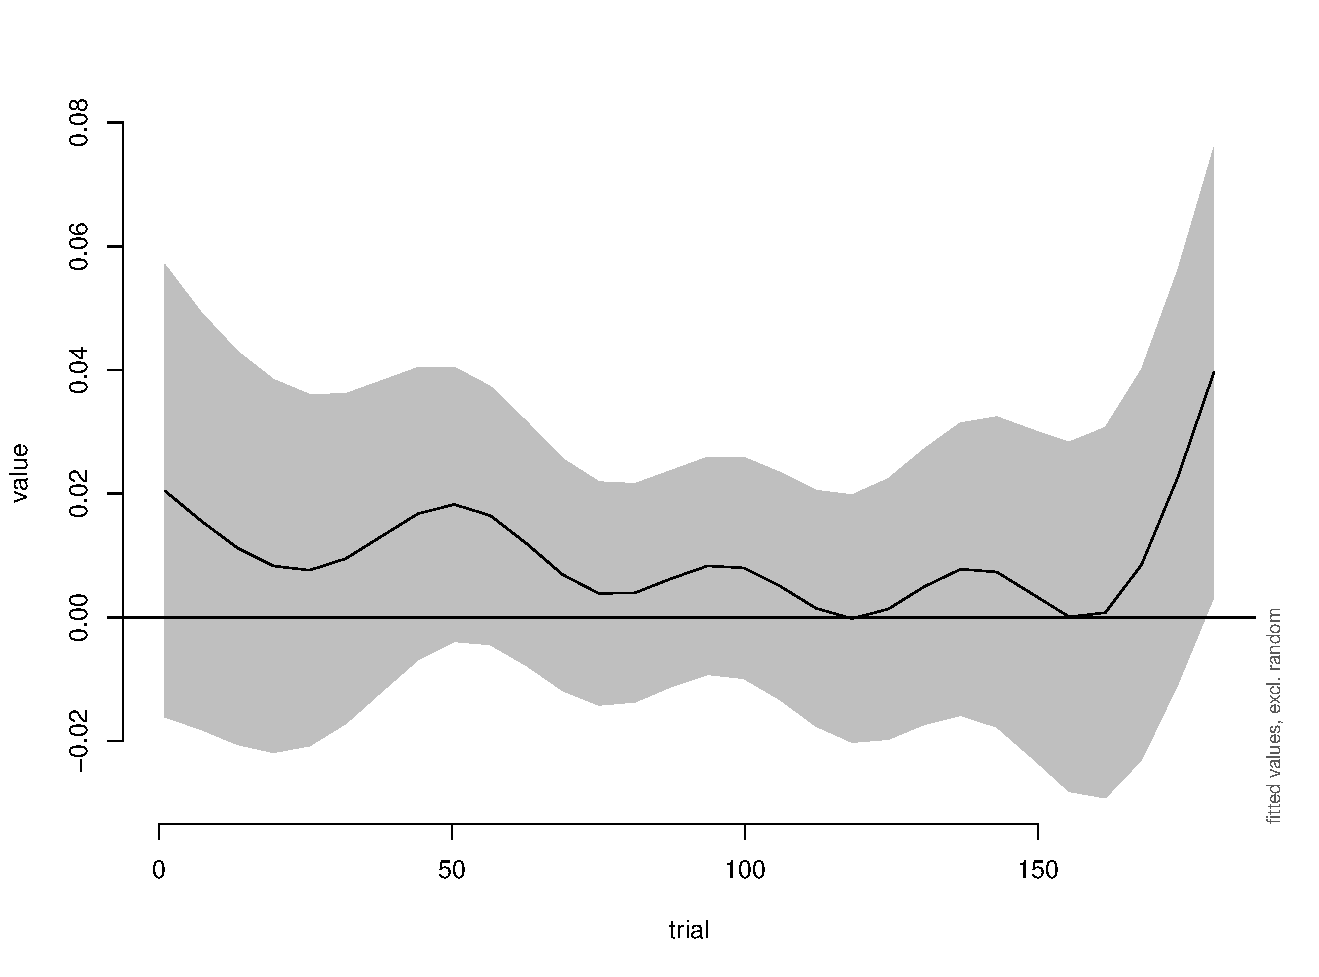
\includegraphics[width=\linewidth]{../stats/results/imagcoh-theta.pdf}
  \caption{Predicted imaginary part of coherency without random effects in the theta band.}
  \label{fig:imagcohtheta}
\end{figure}

\begin{figure}[!htpb]
  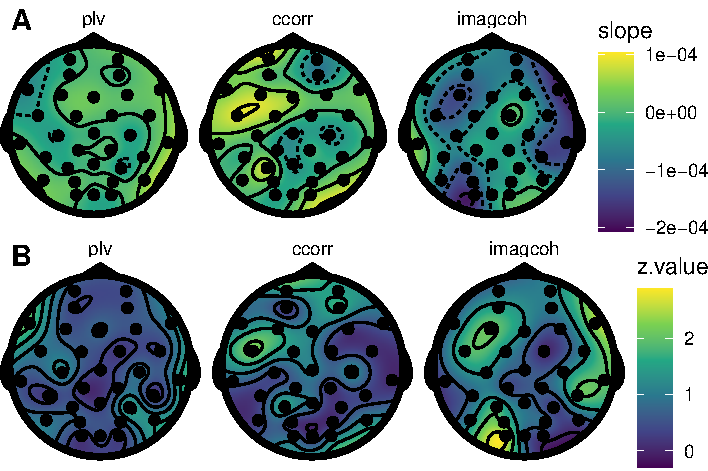
\includegraphics[width=\linewidth]{../stats/results/slopes_theta.pdf}
  \caption{One inter-brain synhrony value is calculated per trial in the theta band. (A) shows their (average) slope when we fit a line through them. (B) shows none of these slopes are significantly different from zero after FDR correction by comparing a linear mixed effect model that includes the slope to one that does not for each electrode.}
  \label{fig:slopes_theta}
\end{figure}

\begin{figure}[!htpb]
  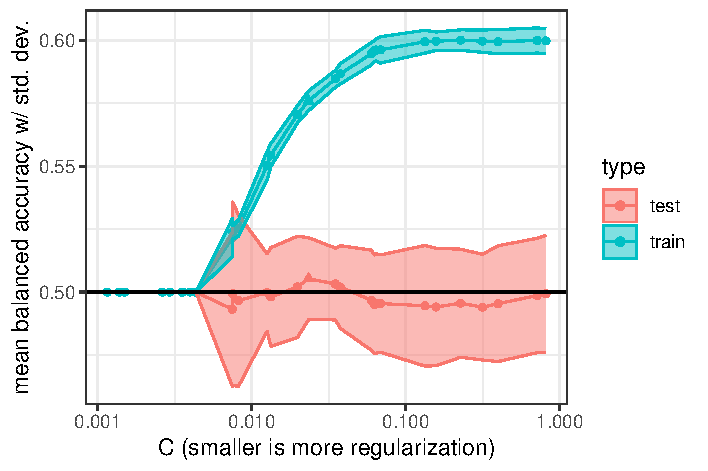
\includegraphics[width=\linewidth]{../stats/results/learning_curve_logistic.pdf}
  \caption{Logistic regression: performance on the train and test set during cross-validation for different regularization parameters. The triangle shows the parameter used for final evaluation.}
  \label{fig:learning_curve_logistic}
\end{figure}

\begin{figure}[!htpb]
  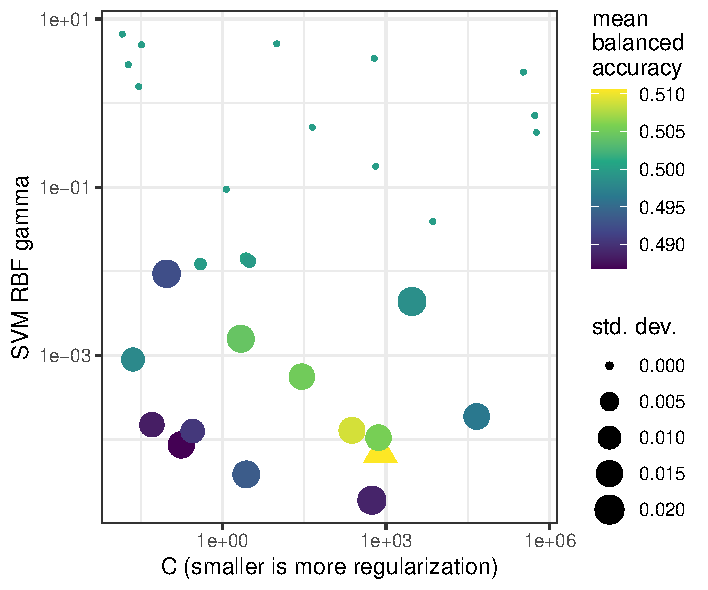
\includegraphics[width=\linewidth]{../stats/results/learning_curve_svm.pdf}
  \caption{SVM: performance on the test set during cross-validation for different regularization and radial basis function size parameters. The triangle shows the parameters used for final evaluation.}
  \label{fig:learning_curve_svm}
\end{figure}

\begin{figure}[!htpb]
  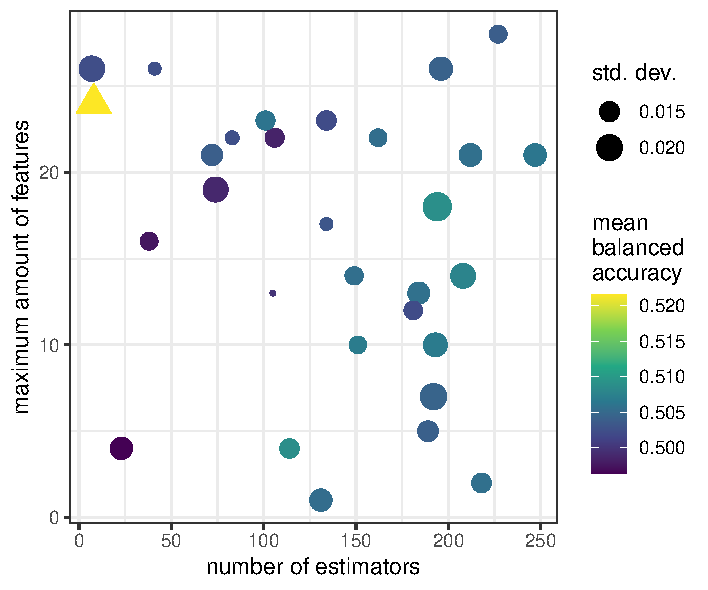
\includegraphics[width=\linewidth]{../stats/results/learning_curve_rf.pdf}
  \caption{Random Forest: performance on the test set during cross-validation for different number of estimators and maximum amounts of features. The triangle shows the parameters used for final evaluation.}
  \label{fig:learning_curve_rf}
\end{figure}

\begin{figure}[!htpb]
  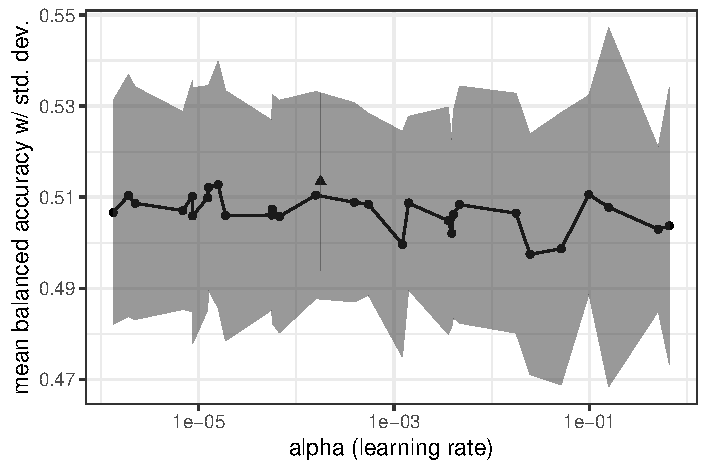
\includegraphics[width=\linewidth]{../stats/results/learning_curve_mlp.pdf}
  \caption{Multi-layer perceptron: performance on the test set during cross-validation for different learning rates. The triangle shows the rate used for final evaluation.}
  \label{fig:learning_curve_mlp}
\end{figure}

\begin{figure}[!htpb]
  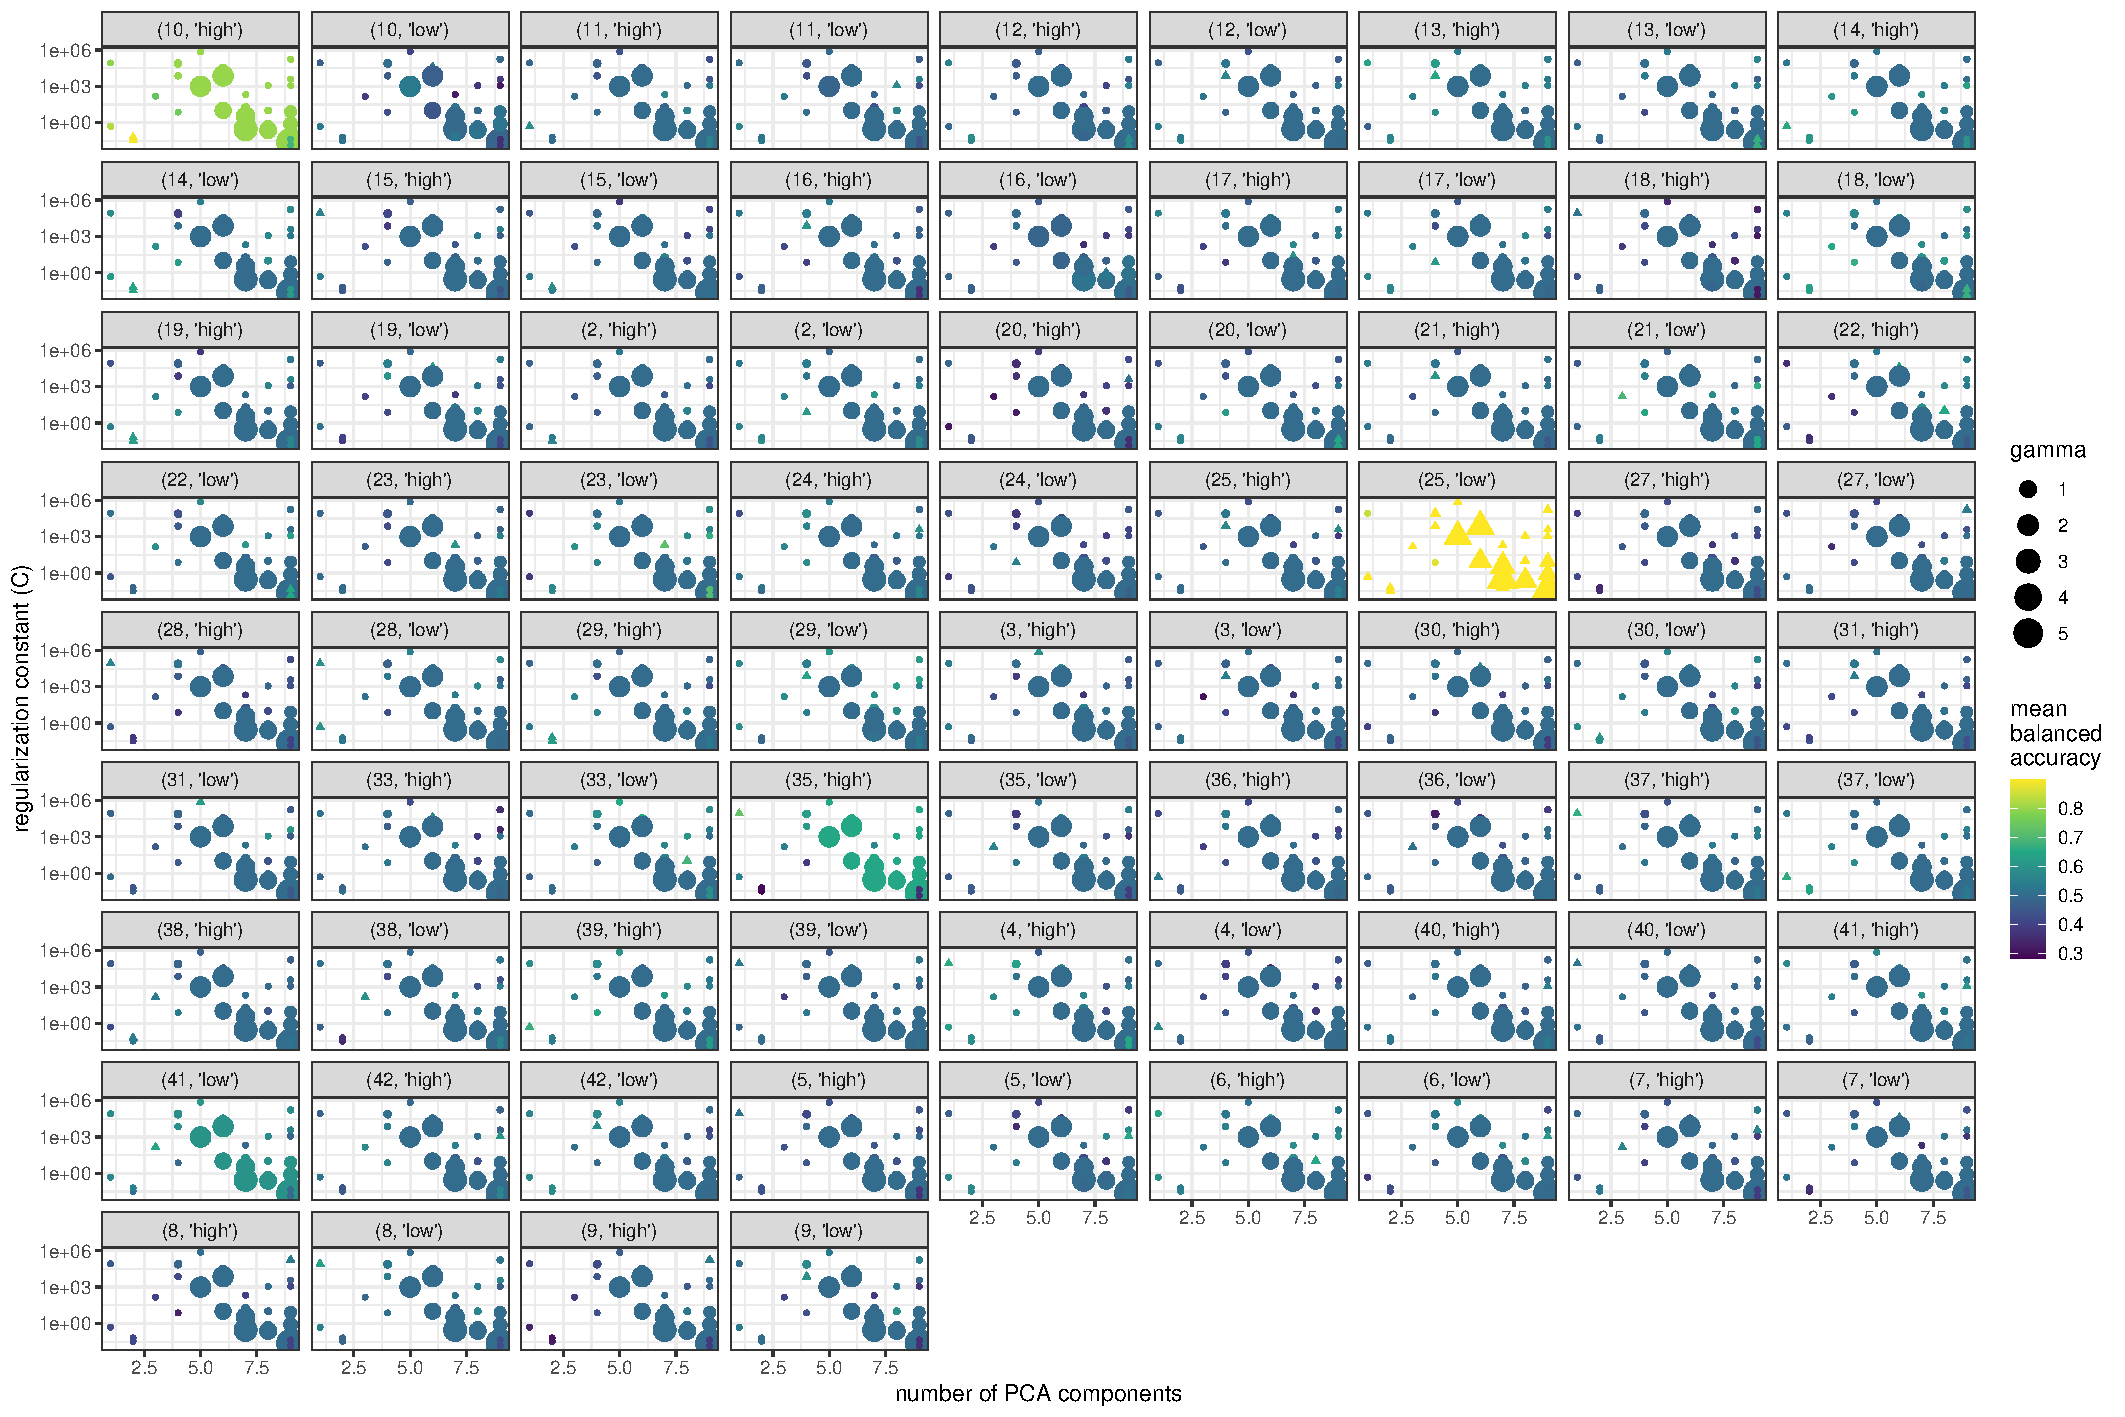
\includegraphics[angle=90,width=.95\linewidth]{../stats/results/learning_curve_within_dyad.pdf}
  \caption{Within-dyad SVM classifiers: performance on the test set during cross-validation for different regularization and SVM RBF gamma parameters. A triangle shows the parameters used for final evaluation. One plot for each session and WM manipulation.}
  \label{fig:learning_curve_within_dyad}
\end{figure}

\nocite{de_vries_marten--vriesmeasuring-inter-brain-synchrony_2022}
\printbibliography
\end{document}
